
\documentclass[11pt,a4paper,fleqn,openany]{report}

\usepackage{analysis_3_sty}
\input{analysis_3_skript_cfg.tex}

\begin{document}
  \sidenote{Vorlesung 1}{02.11.2020}
  % 
  % Vorwort
  % 
  \begin{goals}
    \begin{enumerate}
      \item[]
      \item Maßtheorie $\to$ Lebesgue-Maß\\(Volumen von Teilmengen des $\mathbb{R}^n$ bestimmen)
      \item Integralrechnung für Funktionen $f:\Omega \subseteq \mathbb{R}^n \to \mathbb{R}$\\$\to$ Lebesgue-Integrale (Satz von Fubini, ...)
      \item Version des Hauptsatzes $\to$ Satz von Gauß 
    \end{enumerate}
  \end{goals}

  \input{chapter1}
  \input{chapter2}
  \input{chapter3}
  \chapter{Lebesgue-Integral}
  \begin{definition}
    $X$ Menge, $\mu$ äußeres Maß. Eine funktion $\zeta: X \to \mathbb{R}$ heißt $\bm{\mu}$\textbf{-Treppenfunktion}, wenn sie $\mu$-messbar ist und nur eindlich viele Funktionswerte annimmt.\\
    Die Menge $\script{T}(\mu)$ der $\mu$-Treppenfunktionen ist ein $\mathbb{R}$-Vektorraum. Wir setzen
    \begin{align*}
      \script{T}^+(\mu)=\{\zeta \in \script{T}(\mu) \ | \ \zeta \geq 0\}
    \end{align*}
  \end{definition}

  \begin{example}
    $E \subseteq X, \psi_E: X \to \mathbb{R}, \psi_E(x) = \begin{cases}
      1 & ,x \in E\\
      0 & ,\text{ sonst}
    \end{cases}$  Es ist: $\psi_E$ $\mu$-Treppenfunktion $\Leftrightarrow E \in \script{M}(\mu)$\\
    Sei $\zeta \geq 0, \zeta = \sum\limits_{i=1}^k s_i \psi_{A_i}$ mit $A_i$ messbar und $s_i \geq 0$ und die $A_i$ sind paarweise disjunkt. So eine Darstellung heißt \textbf{einfach}.\\
    Wir setzen:
    \begin{align*}
      (\star) \ I(\zeta) := \sum\limits_{i=1}^k s_i \mu(A_i)
    \end{align*} 
    Für $\zeta=0$ folgt $I(\zeta) = 0 \cdot \mu(X) = 0$\\
    Jedes $\zeta \in \script{T}^+(\mu)$ besitzt eine einfache Darstellung, z.B. können wir für $s_i$ die endlich vielen Funktionswerte wählen und $A_i = \{\zeta = s_i\}$
  \end{example}

  \begin{lemma}
    Das Integral $I: \script{T}^+(\mu) \to [0,\infty]$ ist durch $(\star)$ wohldefiniert. Für $\zeta, \phi \in \script{T}^+(\mu)$ und $\alpha, \beta \in [0, \infty)$ gilt:
    \begin{enumerate}[label=\roman*)]
      \item $I(\alpha \zeta + \beta \psi) = \alpha I(\zeta) + \beta I(\psi)$
      \item $\zeta \leq \psi \implies I(\zeta) \leq I(\psi)$ 
    \end{enumerate}
  \end{lemma}

  \begin{proof}
    Sei $\zeta = \sum\limits_{i=1}^{k} s_i \psi_{A_i}$ einfach $\implies \{\zeta > 0\} = \bigcup\limits_{i;s_i >0} A_i$.\newline
    Ist $\mu (\{ \zeta >0\}) = \infty$ $\implies s_i \mu (A_i) = \infty$ für mindestens ein $i$ und damit $I(\zeta )= \infty$. \newline
    Sei nun $\mu(\{\zeta\}) < \infty$ und $\zeta = \sum\limits_{j=1}^l t_j \psi_{B_j}$ eine zweite einfache Darstellung. \newline
    z.z. $\sum\limits_{i=1}^k s_i \mu (A_i) = \sum\limits_{j=1}^l t_j \mu (B_j)$ \newline
    $\implies I$ wohldefiniert $\implies A_i\cap B_j$ sind messbar und paarweise disjunkt und es gilt \newline
    $0 = \sum\limits_{i=1}^k s_i \psi_{A_i} - \sum\limits_{j=1}^l t_j \psi_{B_j} = \sum\limits_{i=1}^k \sum\limits_{j=1}^l (s_i - t_j )\psi_{A_i \cap B_j}$. \newline
    Für $A_i \cap B_j \neq \varnothing \implies s_i = t_j$ \newline $ \implies \sum\limits_{i=1}^{k} s_i \mu (A_i) - \sum\limits_{j=1}^l t_j \mu (B_j) = \sum\limits_{i=1}^k \sum\limits_{j=1}^l (s_i - t_j)\mu (A_i\cap B_j)=0$ \newline
    Sei nun $\zeta = \sum\limits_{i=1}^k s_i \psi_{A_i}$, $\Psi = \sum\limits_{j=1}^l t_j \psi_{B_j}$ einfache Darstellungen von $\zeta$,$\psi\in \script{T}^+(\mu) \\ \implies \alpha \zeta + \beta \Psi = \sum\limits_{i=1}^k \sum\limits_{j=1}^l (\alpha s_i + \beta t_j)\psi_{A_i\cap B_j}$. Das ist einfach. \newline
    $\implies I(\alpha \zeta + \beta \Psi) = \sum\limits_{i=1}^k \sum\limits_{j=1}^l (\alpha s_i + \beta t_j) \mu (A_i \cap B_j) = \alpha I(\zeta) + \beta I(\Psi) \implies$ i) \newline
    In ii) gilt $\Psi - \zeta \in \script{T}^+(\mu)$ und damit $I(\Psi) = I(\zeta + (\Psi - \zeta)) \overset{i)}{=} I(\zeta) + I(\Psi - \zeta) \geq I(\zeta)$
    
  \end{proof}

  \begin{remark}
    Für $A_i$ messbar und $s_i \geq 0$ folgt aus i) auch für $A_i$ nicht disjunk:
    \begin{align*}
      I(\zeta) = \sum\limits_{i=1}^k s_i \mu(A_i) \ \ \text{ für } \zeta = \sum\limits_{i=1}^k s_i \psi_{A_i}
    \end{align*}
  \end{remark}

  \begin{definition}[Lebesgue-Integral]
    Für $f: X \to [0,\infty]$ $\mu$-messbar, setze
    \begin{align*}
      \int f d\mu = sup\{I(\zeta) \ | \ \zeta \in \script{T}^+(\mu), \zeta \leq f\}
    \end{align*}
    $\zeta$ heißt \textbf{Unterfunktion} von f.\\
    Ist $f: X \to [-\infty, \infty]$ $\mu$-messbar und sind die Integrale von $f^{\pm}$ nicht beide unendlich, so setzen wir
    \begin{align*}
      \int f d\mu = \int f^+ d\mu - \int f^- d\mu \ \ \in [-\infty, \infty] 
    \end{align*}
  \end{definition}

  \begin{remark}
    Für $f \geq 0$ sind beide Schritte kompatibel, denn dann gilt $f = f^+$ und $f^- = 0$
  \end{remark}

  \begin{lemma}
    Für $f \in \script{T}^+(\mu)$ gilt: $\int f d\mu = I(f)$
  \end{lemma}

  \begin{proof}
    $f$ ist Unterfunktion von $f$ $\implies \int f d\mu \geq I(f)$. \newline
    Lemma IV.2 ii) $\implies I(\zeta) \leq I(f)$ $\forall \zeta$ Unterfunktion von f $\implies \int f d\mu \leq I(f)$.
  \end{proof}

  \begin{example}
    $\chi_{\mathbb{Q}}$ ist eine $\lambda^1$-Treppenfunktion und es gilt:\\
    $\int \chi_{\mathbb{Q}} d\lambda^1 = I(\chi_{\mathbb{Q}}) = 0 \cdot \lambda^1(\mathbb{R} \setminus \mathbb{Q}) + 1 \cdot \lambda^1(\mathbb{Q}) = 0 + 1 \cdot 0 = 0$
  \end{example}

  \begin{definition}
    $f:X \to \bar{\mathbb{R}}$ heißt \textbf{integrierbar} bzgl. $\mu$, wenn sie $\mu$-messbar ist und wenn gilt:
    \begin{align*}
      \int f d\mu \in \mathbb{R} \Leftrightarrow \int f^+ d\mu + \int f^- d\mu < \infty
    \end{align*}
  \end{definition}

  \begin{example}
    $\mu = card, X = \mathbb{N}_0$\\
    z.z.: $f: \mathbb{N}_0 \to \mathbb{R}$ ist bzgl. $card$ auf $\mathbb{N}_0$ integrierbar $\implies \sum\limits_{k \in \mathbb{N}} f(k)$ absolut konvergent\\
    Dann gilt: $\int f d card = \sum\limits_{k \in \mathbb{N}} f(k)$\\
    
    i) $f: \mathbb{N}_0 \to [0,\infty]$ \\
    Betrachte $f_n: \mathbb{N}_0 \to \mathbb{R}$, $f_n(k) = \begin{cases} f(k) \text{ ,}k\leq n \\ 0\text{ sonst } \end{cases}$ \\
    $f_n$ sind Unterfunktionen von $f$ mit $I(f_n)=\sum\limits_{k=0}^nf(k) \\ \implies \int f dcard \geq \lim\limits_{n\to\infty} I(f_n) = \sum\limits_{k=0}^{\infty} f(k)$\\
    Umgekehrte Abschätzung: \\
    Dazu sei O.E. $\sum\limits_{k=0}^\infty f(k) <\infty \implies f(k)\to 0$ mit $k\to\infty$ \\
    $\zeta$ Unterfunktion von $f$, so ist $\zeta (k) \neq 0$ nur für endlich viele $k$ und damit $\zeta \leq f_n$ für $n$ hinreichend groß. \\
    $\implies I(\zeta)\leq I(f_n) = \sum\limits_{k=0}^n f(k)\leq \sum\limits_{k=0}^\infty f(k)$ \\
    $\implies \int f dcard \leq \sum\limits_{k=0}^\infty f(k)$ \\
    
    Äquivalend von Integrierbarkeit und absolute Konvergenz: \\
    $\inf f^+ dcard + \inf f^- dcard = \sum\limits_{k=0}^\infty f^+(k)+\sum\limits_{k=0}^\infty f^-(k) = \sum\limits_{k=0}^\infty |f(k)|$ \\
    Und weiter \\
    
    ii) $f: \mathbb{N}_0 \to \mathbb{\bar{R}}$ \\
    $\int f dcard = \inf f^+ dcard - \int f^- dcard = \sum\limits_{k=0}^\infty f^+(k) - \sum\limits_{k=0}^\infty f^-(k) = \sum\limits_{k=0}^\infty f(k)$
  \end{example}
  \newpage
  \begin{theorem}
    $f,g:X \to \bar{\mathbb{R}}$ $\mu$-messbar. Ist $f \leq g$ $\mu$-fast überall und $\int f^- d\mu < \infty$, so existieren beide Integrale und es ist: $\int f d\mu \leq \int g d\mu$\\
    \glqq$\geq$\grqq gilt entsprechend wenn $f^+ d\mu < \infty$
  \end{theorem}

  \begin{proof}
    \item[i)] $f,g \geq 0$. Ist $\zeta = \sum\limits_{i=1}^k s_i \psi_{A_i}$ Unterfunktion von $f$ $\implies \Psi := \psi_{\{f \leq g \}}\zeta = \sum\limits_{i=1}^k s_i \psi_{\{f\leq g\}\cap A_i}$ Unterfunktion von g \\
    $\implies I(\zeta) = \sum\limits_{i=1}^k s_i \mu (A_i) = \sum\limits_{i=1}^k s_i \psi(\{f \leq g\}\cap A_i) = I(\Psi) \leq \int g d\mu$ \\
    $\implies\int f d\mu \leq \int g d\mu$ 
    \item[ii)] $f,g$ beliebig. \\
    Es gilt: $f^+ > 0 \implies f= f^+$ \\
    $f^+ > g^+ \implies f = f^+ > g^+ \geq g \\
    f^- < g^- \implies f \geq f^- > -g^- = g$ \\
    Aus $f \leq g$ folgt $f^+ \leq g^+$ und $f^- \geq g^-$ fast überall. \\
    $\implies \int f^+ d\mu \leq \int g^+ d\mu$, $\infty > \int f^- d\mu \geq \int g^- d\mu \\ 
    \implies \int f d\mu = \int f^+ d\mu - \int f^- d\mu \leq \int g^+ d\mu - \int g^- d\mu = \int g d\mu$
    
  \end{proof}

  \begin{remark}
    $f,g: X \to \bar{\mathbb{R}}$, $f$ $\mu$-messbar und $g = f$ $\mu$-fast überall $\stackrel{\text{Kapitel II}}{\implies} g$ $\mu$-messbar\\
    Satz IV.6 $\implies \int g^{\pm} d\mu = \int f^{\pm} d\mu \implies \int f d\mu = \int g \ d\mu$
  \end{remark}

  \sidenote{Vorlesung 12}{11.11.2020}

  \begin{remark}
    Einschub: zum Beweis von Satz III.7 \\
    $D$ $\lambda^n$-messbar \\ 
    Schreibe $D = \bigcup\limits_{j=1}^\infty D_j$ mit $D_j = \{x\in D: j-1 \leq ||x|| < j\}$ \\
    Lemma III.6 $\implies \exists U_{i,j}$ offen bzw. $K_{i,j}$ kompakt mit $K_{i,j}  \subset D_j \subset U_{i,j}$ und \\ $\lambda^n (U_{i,j}) < \lambda^n (D_j) + \frac{2^{-j}}{i}$, $\lambda^n (K_{i,j}) > \lambda^n (D_j) - \frac{2^{-j}}{i}$ \\
    $\implies U_i := \bigcup\limits_{j=1}^\infty U_{i,j}$ offen und $A_i := \bigcup\limits_{j=1}^\infty K_{i,j}$ abgeschlossen.
  \end{remark}
  \begin{example}
  	$K_n = \{\frac{1}{n}\}$, $\bigcup\limits_{n=1}^\infty \{ \frac{1}{n}\}$ nicht abgeschlossen. \\
  	\item[Beweis] Sei $x\in \bar{A}_i \implies \exists K\subset \mathbb{R}^n$ kompakt mit $x\in $\r{K} (z.B. $K = \overline{B_{\frac{1}{2}}(x)}$). \\
  	$\implies \exists x_n \in A_i$ mit $x_n \to x$ O.E. $x_n \in A_i\cap K$ \\
  	$K$ schneidet höchstens endlich viele $K_{i,j}$ \\ 
  	endliche Vereinigung von diesen $K_{i,j}$ und $K$ ist abgeschlossen \\
  	$\implies x\in A_i \implies A_i = \overline{A_i} \implies A_i$ abgeschlossen.
  \end{example}

  \begin{lemma}[Tschebyscheff-Ungleichung]
    Für $f:X \to [0, \infty]$ $\mu$-messbar mit $\int f d\mu < \infty$ gilt:
    \begin{align*}
      \mu(\{f\geq s\}) \leq \begin{cases}
        \dfrac{1}{s} \cdot \int f d\mu & \text{ für } s \in (0, \infty)\\
        0 & \text{ für } s = \infty
      \end{cases}
    \end{align*}
  \end{lemma}

  \begin{proof}
    Für $s \in (0,\infty)$ ist $s \psi_{}\ f \geq s {\}}$ eine Unterfunktion von $f$ \\ $\implies s \mu (\{f = \infty\}) \leq s \mu (\{f\geq s \}) = I(s\psi_{\{f\geq s\}}) \leq \int f d\mu$
  \end{proof}

  \begin{lemma}
    Sei $f: X \to \bar{\mathbb{R}}$ $\mu$-messbar.
    \begin{enumerate}[label=\roman*)]
      \item ist $\int f d\mu < \infty \implies \{f = \infty\}$ ist $\mu$-Nulllmenge
      \item ist $f \geq 0$ und $\int f d\mu = 0 \implies \{f > 0\}$ ist $\mu$-Nullmenge
    \end{enumerate}
  \end{lemma}

  \begin{proof}
    \item[i)] Folgt mit $s=\infty$ aus Lemma IV.7 angewand auf $f^+$
    \item[ii)] Lemma IV.7 $\implies \mu(\{f\geq s\})=0$ für $s>0$ $\overset{\text{Lemma II.8}}{\implies} \mu(\{f >0\})=0$
  \end{proof}

  \begin{theorem}
    Zu $f: X \to [0,\infty]$ $\mu$-messbar gibt es eine Folge $f_k \in \script{T}^+(\mu)$ mit $f_0 \leq f_1 \leq ...$ und $\lim\limits_{k \to \infty} f_k(x) = f(x) \ \forall x \in X$.
  \end{theorem}

  \begin{proof}
    Sei $c_k > 0$ eine Nullfolge mit $\sum\limits_{k=1}^\infty c_k = \infty$ (z.B. $c_k = \frac{1}{k}$) \\
    Setze $f_0 := 0$ und definiere für $k\geq 1$ induktiv $E_k = \{f_{k-1}+c_k \leq f  \}$ sowie  \\ $f_k = f_{k-1}+c_k\psi_{E_k} \implies f_k = \sum\limits_{j=1}^k c_j\psi_{E_j}$ \\
    $\implies f_k$ sind Treppenfunktionen mit $f_0 \leq f_1 \leq ...$ und $f_k \leq f$ $\forall$ $k\in\mathbb{N}$. Denn ist $x\in E_k$, so gilt $f_k(x) = f_{k-1}(x)+c_k \leq f(x)$ nach Definition. \\
    Ist $x \notin E_k \implies f_k(x) = f_{k-1}(x) \leq f(x)$. \\
    Nach Induktion $\implies \lim\limits_{j\to\infty} f_k(x) \leq f(x)$ $\forall x\in X$. \\
    Sei $\lim\limits_{l\to\infty} < \infty $. Da $\sum\limits_{k=1}^\infty c_k = \infty$ existiert $\infty$-viele $k\in\mathbb{N}$ mit $x\notin E_k$. \\
    $\implies f_{k-1}(x) > f(x)-c_k$  für $\infty$-viele $k$ $\implies \lim\limits_{k\to\infty}f_k(x) \geq f(x)$
  \end{proof}

  \newpage
  \begin{theorem}[Monotonie Konvergenz / Beppo-Levi]
    Seien $f_k:X \to [0,\infty]$ $\mu$-messbar mit $f_1 \leq f_2 \leq ...$ und $f: X \to [0, \infty]$ mit $f(x) := \lim\limits_{k \to \infty} f_k(x)$. Dann gilt:
    \begin{align*}
      \int f d\mu = \lim\limits_{k \to \infty} \int f_k \ d\mu
    \end{align*}
  \end{theorem}

  \begin{proof}
	Seien $f$ ist $\mu$-messbar nach Satz I.16. Mit Satz IV.6 gilt: \\ 
	$0 \leq \int f_1 d\mu \leq \int f_2 d\mu \leq ... \leq \int f d\mu \implies \lim\limits_{k\to\infty} \int f_k d\mu \leq \int f d\mu$ \\
	Sei $\zeta$ Unterfunktion von $f$ mit Wertemenge $\{s_1, ..., s_m\}$. Setze $E_i = \{\zeta = s_i\}$ für $i=1,...,m$. \\ 
	Betrachte für $\Theta \in (0,1)$ die Mengen $E_{i,k} = E_i \cap \{f_k \geq \Theta s_i\} $ \\
	$\implies \sum\limits_{k=1}^m \Theta s_i \psi_{E_i,k}$ ist Unterfunktion von $f_k$ \\
	$\overset{\text{Lemma IV.2}}{\implies} \sum\limits_{i=1}^m \Theta s_i \mu (E_{i,k}) = I(\sum\limits_{i=1}^m \Theta_i s_i \psi_{E_{i,k}})\leq \int f_k d\mu$ \\
	Jetzt gilt: $E_i = \bigcup\limits_{k=1}^\infty E_{i,k}$, denn für $s_i > 0$ ist $\lim\limits_{k\to\infty} f_k(x) = f(x)$ $\forall x\in E_i$. \\ 
	Außerdem: $E_{i,1} \subset E_{i,2} \subset ..." \overset{\text{Satz I.7}}{\implies} \mu (E_i) = \lim\limits_{k\to\infty}\mu (E_{i,k})\\ 
	\implies \Theta I(\zeta) = \sum\limits_{i=1}^m \Theta s_i \mu (E_i) = \lim\limits_{k\to\infty}^m \Theta s_i \mu (E_{i,k}) \leq \lim\limits_{k\to\infty} \int f_k d\mu$ \\
	Mit $\Theta \to 1$ und nach Bildung des Supremums über alle Unterfunktionen $\zeta$ gilt: \\ $\int f d\mu \leq \lim\limits_{k\to\infty} \int f_k d\mu$.
  \end{proof}

  \begin{theorem}
    $f,g: X \to \bar{\mathbb{R}}$ integrierbar bzgl. $\mu$, so ist auch $\alpha f + \beta g$ integrierbar $\forall \alpha, \beta \in \mathbb{R}$ und es gilt:
    \begin{align*}
      \int (\alpha f + \beta g) \ d\mu = \alpha \int f d\mu + \beta \int g d\mu
    \end{align*}
  \end{theorem}

  \begin{proof}
    \item[I.] $f\geq 0$, $\alpha > 0$ $\implies \int (\alpha f) d\mu = \alpha \int f d\mu$. \\
    Sei dazu $\zeta$ Unterfunktion von $f$ $\implies \alpha \zeta$ ist Unterfunktion von $\alpha f$ und mit Lemma IV.2 folgt: $\alpha I(\zeta) = I(\alpha \zeta) \leq \int (\alpha f) d\mu$. Also: $\alpha \int f d\mu \leq \int (\alpha f) d\mu$. \\
    Ersetze $\alpha$ durch $\frac{1}{\alpha}$ von $f$ durch $(\alpha f) \implies \alpha \int f d\mu \geq \int (\alpha f) d\mu$. 
    \item[II.] $f$ integrierbar, $\alpha > 0$ $\implies \alpha \int f d\mu = \int (\alpha f) d\mu$. \\ Denn $(\alpha f)^\pm = \alpha f^\pm \\ \implies \int (\alpha f) d\mu = \int (\alpha f)^+ d\mu - \int (\alpha f)^- d\mu \overset{\text{I}}{=} \alpha \int f^+ d\mu - \alpha \int f^- d\mu = \alpha \int f d\mu$.
    \item[III.] $\int (-f) d\mu = -\int f d\mu$, denn $(-f)^\pm = f^\mp \\ \implies \int (-f) d\mu = \int (-f)^+ d\mu - \int (-f)^- d\mu = \int f^- d\mu - \int f^+ d\mu = -\int f d\mu$ \\
    \item[z.z.] Linearität für $f+g$ 
    \item[i)]$f,g \geq 0$ \\
    Satz IV.9 $\implies \exists \zeta_k,\Psi_k \in \script{T}^+(\mu)$ mit $\zeta_k \to f$, $\Psi_k \to g$ punktweise.$\implies \zeta_k + \Psi_k \to f+g$ \\
    Satz IV.10 und Lemma IV.2 \\
    $\int (f+g) d\mu = \lim\limits_{k\to\infty} \int (\zeta_k +\Psi_k ) d\mu = \lim\limits_{k\to\infty}(\int \zeta_k d\mu + \int \Psi_k d\mu) = \int f d\mu + \int g d\mu$ 
    \item[ii)] $f,g: X\to\mathbb{R}$ integrierbar \\
    Betrachte $\phi = f^+ + g^+ - (f+g)^+ \geq 0$, $\psi = f^- + g^- -(f+g)^- \geq 0$ \\
    $\implies \phi-\psi = f^+ - f^- +g^+-g^--(f+g)^++(f+g)^- = f+g-(f-g) = 0 \\
    \implies \int (f^+ + g^+) d\mu \overset{\text{i)}}{=} \int (f+g)^+ d\mu + \int \phi d\mu $ \\
    $\implies \int (f^- + g^- )d\mu \overset{\text{i)}}{=} \int (f+g)^- d\mu + \int \psi d\mu$ \\
    $\implies$ Beh.
    \item[iii)] $f,g: X\to\mathbb{\bar{R}}$ \\
    O.E. $\int f d\mu + \int g d\mu > -\infty.$ \\ 
    Also $\int f^- d\mu + \int g^- d\mu < \infty$. \\ 
    (Sonst gehe zu $-f$, $-g$ über und benutze den ersten Teil mit $\alpha = -1$) \\
    Lemma IV.8 $\implies \mu(\{f=-\infty \} \cup \{g = -\infty \}) =0\implies \{(f,g) = \pm (\infty,-\infty)  \}\in \script{M}(\mu)$ ist eines $\mu$-Nullmenge. \\
    Aus $(f+g)^- \leq f^- + g^-$ und Monotonie folgt: \\
    $\int (f+g)^- d\mu \leq \int (f^- + g^-) d\mu \overset{\text{i)}}{=} \int f^- d\mu + \int g^- d\mu < \infty \implies \int (f+g) d\mu$ ist definiert. \\
    Es gilt: \\
    $(f+g)^+ - (f+g)^- = f+g = f^+ + g^+ -(f^- + g^- )$ bzw. \\
    $(f+g)^+ + f^- +g^- = (f+g)^- +f^+ + g^+ \\
    \overset{\text{i)}}{\implies} \int (f+g)^+ d\mu + \int f^- d\mu + \int g^- d\mu = \int (f+g)^- d\mu + \int f^+ d\mu + \int g^+ d\mu$.\\
    Ist $\int f^+ d\mu + \int g^+ d\mu < \infty$, so sind alle Integrale endlich und \\ $\int (f+g) d\mu = \int (f+g)^+ d\mu - \int (f+g)^- d\mu = \int f^+ d\mu + \int g^+ d\mu - \int f^- d\mu - \int g^- d\mu = \int f d\mu + \int g d\mu$. \\
    Ist $\int f^+ d\mu + \int g^+ d\mu = \infty \implies \int (f+g)^+ d\mu = \infty \\ \implies \int (f+g) d\mu = \infty = \int f d\mu + \int g d\mu$
  \end{proof}

  \begin{definition}
    Sei $\mu$ ein äußeres Maß auf $X$ und $E \subseteq X$ sei $\mu$-messbar. Dann setzen wir, falls das rechte Integral existiert
    \begin{align*}
      \int\limits_E f d\mu = \int f \chi_E d\mu
    \end{align*}
    $f$ heißt \textbf{auf $\bm{E}$ integrierbar}, wenn $f \chi_E$ integrierbar ist.
  \end{definition}

  \begin{remark}
    Wegen $(f \chi_E)^{\pm} = f^{\pm} \chi_E \leq f^{\pm}$ existiert das Integral von $f$ über $E$ auf jeden Fall dann, wenn $\in f d\mu$ existiert. (Speziell für $f \geq 0$)
  \end{remark}

  \begin{example}
    $\alpha \in \mathbb{R}, \ f:\mathbb{R}^n \to \mathbb{R}, \ f(x) = ||x||^{-\alpha}$\\
    Beh: 
    \begin{align*}
      \int\limits_{\mathbb{R}^n \setminus B_1(0)} f d\lambda^n < \infty &\Leftrightarrow \alpha > n\\
      \int\limits_{B_1(0)} f d\lambda^n < \infty &\Leftrightarrow \alpha < n
    \end{align*}
    Vergleiche dazu $f$ mit $g = \sum\limits_{k\in\mathbb{Z}} 2^{-k \alpha} \psi_{A_k}$, $A_k = \{2^k \leq ||\alpha|| < 2^{k+1}  \}$ \\
    Es gilt: \\
    $2^{-\alpha} g \leq  f \leq g$ für $\alpha > 0$ \\
    $2^{-\alpha} g \geq f \geq g$ für $\alpha \leq 0$ \\ 
    Monotonie $\implies$ Reicht die Aussagen für $g$ zu zeigen. \\
    $A_k = 2^k A_0, Y_n := \lambda^n (A_0) \in (0,\infty) \\
    \overset{\text{Satz III.16}}{\implies} \lambda^n (A_k) = (2^l) \lambda^n(A_0) = 2^{nk}Y_n\\
    \sum\limits_{k=0}^l 2^{-k\alpha}\psi_{A_k}$ konv. punktweise auf $\mathbb{R}^n$ gegen $g\psi_{\mathbb{R}^n\setminus B_1(0)}$. Folge ist monoton wachsend. \\
    $\overset{\text{Satz über Mon. Konvergenz}}{\implies} \int\limits_{\mathbb{R}^n\setminus B_1(0)} g d\lambda^n = \sum\limits_{k=0}^\infty \int 2^{-k\alpha}\psi_{A_k} d\lambda^n = Y_n \sum\limits_{k=0}^\infty 2^{n-\alpha)k} = \begin{cases}Y_n \frac{1}{1-2^{n-\alpha}} \text{falls } \alpha \geq n \\ \infty \text{ sonst } \end{cases}$ \\
    Entsprechend gilt auf $B_1(0)$ \\
    $\int\limits_{B_1(0)}g d\lambda^n = \sum\limits_{-\infty}^\infty \int 2^{-k\alpha}\psi_{A_k} d\lambda^n = Y_n \sum\limits_{k=-1}^\infty 2^{(n-\alpha)k} = \begin{cases} Y_n \frac{1}{2^{n-\alpha}-1} \text{ falls } \alpha < n \\ \infty \text{ sonst }\end{cases}$
  \end{example}

  \sidenote{Vorlesung 13}{14.12.20}
  \begin{theorem}
    Sei $f: X \to \bar{\mathbb{R}}$ $\mu$-messbar. Dann gelten:
    \begin{enumerate}[label=\roman*)]
      \item $f$ integrierbar $\Leftrightarrow |f|$ integrierbar
      \item Es gilt: $|\int f d\mu| \leq \int |f| d\mu$, falls das Integral von $f$ existiert
      \item Ist $g: X \to [0, \infty]$ $\mu$-messbar mit $|f| \leq g$ $\mu$-fast überall und $\int g d\mu < \infty$, so ist $f$ integrierbar 
    \end{enumerate}
  \end{theorem}

  \begin{proof}
    Es gilt $|f| = f^+ + f^-$ und Satz IV.11 impliziert $\int |f| d\mu = \int (f^+ + f^-) d\mu = \int f^+ d\mu + \int f^- d\mu \implies \text{i)} $ \\
    Ist $\int f d\mu$ definiert, so gilt $| \int f d\mu | = |\int f^+ d\mu - \int f^- d\mu | \leq \int f^+ d\mu + \int f^- d\mu = \int |f| d\mu \implies \text{ii)}$ \\
    Sei $g$ wie in iii) $\overset{\text{Satz IV.6}}{\implies} \int |f| d\mu \leq \int g d\mu \implies f$ ist integrierbar. 
  \end{proof}

  \begin{example}
    $f: \mathbb{R}^n \to \bar{\mathbb{R}}$ $\lambda^n$-messbar und es gelte für ein $C \in [0, \infty]$:\\
    $|f(x)| \leq C ||x||^{-\alpha}$ fast überall in $B_{\epsilon}(0)$ mit $(\alpha < n)$ bzw.\\
    $|f(x)| \leq C ||x||^{-\alpha}$ fast überall in $\mathbb{R}^n \setminus B_{\epsilon}(0)$ mit $\alpha > n$\\
    $\implies f$ ist auf $B_{\epsilon}(0)$ bzw. $\mathbb{R}^n \setminus B_{\epsilon}(0)$ integrierbar
  \end{example}

  
  \chapter{Konvergenzsätze und $L^n$-Räume}
  \begin{example}
    Punktweise Konvergenz reicht nicht für Konvergenz der Integrale.\\
    Für $\epsilon > 0$ sei $f_{\epsilon}: \mathbb{R} \to \mathbb{R}, f_{\epsilon} = \dfrac{1}{2\epsilon} \chi_{[-\epsilon, \epsilon]}$\\
    Es gilt $f_{\epsilon}(x) = 0$ für $\epsilon < |x|$\\
    $\implies f(x) := \lim\limits_{\epsilon \downarrow 0} f_{\epsilon}(x) = \begin{cases}
      0 & \text{, für } x \neq 0\\
      \infty & \text{, für } x = 0
    \end{cases}$\\
    Weiter $\int f_{\epsilon} d\lambda^1 = \dfrac{1}{2\epsilon} \lambda^1([-\epsilon, \epsilon]) = 1 \ \forall \epsilon > 0$\\
    $\implies \int f d\lambda^1 = 0 < 1 = \lim\limits_{\epsilon \downarrow 0} f_{\epsilon} d\lambda^1$
  \end{example}

  \begin{theorem}[Lemma von Fatou]
    $f_k: X \to [0,\infty]$ Folge von $\mu$-messbaren Funktionen.\\
    Für $f: X \to \bar{\mathbb{R}}, f(x) = \liminf\limits_{k \to \infty} f_k(x)$ gilt:
    \begin{align*}
      \int f d\mu \leq \liminf\limits_{k \to \infty} \int f_k d\mu
    \end{align*}
  \end{theorem}

  \begin{proof}
    Definiere $g_k := \inf\limits_{j\geq k}f_j \implies g_{k+1} \geq g_k$ $\forall k\in\mathbb{N}$ und $\lim\limits_{k\to\infty}g_k = f$ \\
    $\overset{\text{Satz IV.10}}{\implies} \int f d\mu = \lim\limits_{k\to\infty} \int g_k d\mu \leq \liminf\limits_{k\to\infty} \int f_k d\mu$, da $g_k \leq f_k$ $\forall k\in\mathbb{N}$
  \end{proof}

  \begin{theorem}[Dominierte Konvergenz bzw. Satz von Lebesgue]
    $f_1, f_2, ...$ Folge von $\mu$-messbare Funktionen und $f(x) = \lim\limits_{k \to \infty} f_k(x)$ für $\mu$-fast alle $x \in X$. Es gebe eine integrierbare Funktion $g: X \to [0, \infty]$ mit $\sup\limits_{k \in \mathbb{N}} |f_k(x)| \leq g(x)$ für $\mu$-fast alle $x$. Fann ist $f$ integrierbar und $\int f d\mu = \lim\limits_{k \to \infty} \int f_k d\mu$.\\
    Es gilt sogar $||f_k \cdot f||_{L^1(y)} := \int |f_k -f| d\mu \to 0$
  \end{theorem}

  \begin{proof}
    Folge $2g-|f-f_k| \geq 0$ konvergiert punktweise fast überall gegen $2g$. \\
    $\overset{\text{Satz V.i}}{\implies} \limsup |\int f d\mu - \int f_k d\mu | \leq \limsup \int |f-f_k| d\mu \\ = \int 2g d\mu - \liminf \int (2g-|f-f_k|)d\mu \\ \leq 2g d\mu - \int \liminf (2g-|f-f_k|)d\mu = 0$
  \end{proof}

  \begin{remark}[Anwendung]
    Vergleich Riemann-$\int$ mit Lebesgue-$\int$\\
    Sei $I=[a,b]$ kompaktes Intervall, $f:I \to \mathbb{R}$ beschränkt. Unterteilungspunkte $a = x_0 \leq ... \leq x_N = b$ $\to$ Zerlegung $Z$ von $I$ mit Teilintervallen $I_j = [x_{j-1}, x_j]$\\
    $\bar{S}_Z(f) = \sum\limits_{j=1}^N (\sup\limits_{I_j} f) (x_j - x_{j-1}), \ \ \ \underbar{S}_Z(f)= \sum\limits_{j=1}^N (\inf\limits_{I_j} f)(x_j-x_{j-1})$\\
    Für Zerlegungen $Z_1, Z_2$ mit Verfeinerung $Z_1 \cup Z_2$\\
    $\implies \underbar{S}_{Z_1}(f) \leq \underbar{S}_{Z_1 \cup Z_2}(f) \leq \bar{S}_{Z_1 \cup Z_2}(f) \leq \bar{S}_{Z_2}(f)$\\
    $f$ heißt \textbf{Riemann-integrierbar} mit Integral $\int\limits_a^b f(x) dx = S$, falls gilt:\\
    $\sup\limits_Z \underbar{S}_Z(f) = \inf\limits_Z \bar{S}_Z(f) = S$
  \end{remark}

  \begin{theorem}
    $f: I \to \mathbb{R}$ beschränkt auf kompaktem Intervall $I=[a,b]$. Dann gilt:\\
    $f$ Riemann-integrierbar $\Leftrightarrow \lambda^1(\{x \in I \ | \ f \text{ ist nicht stetig in } x\}) = 0$\\
    In diesem Fall ist $f$ auch Lebesgue-integrierbar und die Integrale stimmen überein.
  \end{theorem}

  \begin{proof}
    Für Zerlegung $Z$ mit Teilintervallen $I_j = [x_{j-1},x_j]$, $1\leq j \leq N$.\\ Definiere Riemann-Treppenfunktion: \\ $\bar{f}_z(x) = \max\limits_{x\in I_j}\sup_{I_j} f \geq \limsup\limits_{y\to x} f(y)$, $\underline{f}_z(x) = \min\limits_{x\in I_j}\inf\limits_{I_j} f \leq \liminf\limits_{y\to x} f(y)$.  \\
    Sei $N_f(s) = \{ x\in I: \limsup\limits_{y\to x}f(y) - \liminf\limits_{y\to x}f(y) \geq s \}$ für $s > 0$. \\
    Sind $Z_1$, $Z_2$ bel. Zerlegungen $\implies \bar{f}_{Z_2}(x) - \underline{f}_{Z_1}(x) \geq s$ $\forall x\in N_f(s)$. \\
    $\implies \bar{S}_{Z_2}(f) - \underline{S}_{Z_1}(f) = \int\limits_{I} (\bar{f}_{Z_2}(x)-\underline{f}_{Z_1}(x)) d\lambda^1 \geq s \lambda^1 (N_f(s))$ \\
    Ist $f$ Riemann-integrierbar, so bilde Infimum über alle $Z_1$, $Z_2$ und schließe $\lambda^1 (N_f(s))=0$ $\forall s>0$ $\implies$ "$\implies$". \\
    Sei nun $f$ $\lambda^1$-fast überall stetig und $Z_i$ Folge von Zerlegungen mit Feinheit \\ $\delta_i := \max\limits_{1\leq j \leq N_i} |x_{i,j}-x_{i,j-1}| \to 0$ \\
    Ist $f$ stetig in $x$, so folgt $\bar{f}_{Z_i} (x) \geq \inf\limits_{|y-x| \leq \delta_i } f(y) \to f(x)$ und $\underline{f}_{Z_i} (x) \geq \inf\limits_{|y-x| \leq \delta_i } f(y) \to f(x)$ mit $i\to\infty$ $\implies \bar{f}_{Z_i}$, $\underline{f}_{Z_i}$ konvergiert punktweise $\lambda^1$-fast überall gegen $f$ $\implies f$ ist $\lambda^1$-messbar nach Kapitel I. \\
    Aus $|\bar{f}_{Z_i}|$, $|\underline{f}_{Z_i}| \leq \sup\limits_{I} |f| < \infty$ folgt aus Satz V.2 $\bar{S}_{Z_i}(f) = \int\limits_{I} \bar{f}_{Z_i} d\lambda^1 \to \int\limits_{I} f d\lambda^1$, \\
    $\underline{S}_{Z_i}(f) = \int\limits_{I} \underline{f}_{Z_i} d\lambda^1 \to \int\limits_{I} f d\lambda^1 \implies f$ ist Riemannint. mit $\int\limits_{a}^b f(x) dx = \int\limits_{I} f d\lambda^1$.
  \end{proof}

  \begin{theorem}
    $X$ metrischer Raum, $\mu$ Maß auf $Y$ und $f:X \times Y \to \mathbb{R}$ mit $f(x, \cdot)$ integrierbar bzgl. $\mu \ \forall x \in X$.\\
    Betrachte $F: X \to \mathbb{R}, F(x) = \int f(x,y) d\mu(y)$\\
    Sei $f(\cdot, y)$ stetig in $x_0 \in X$ für $\mu$-fast alle $y \in Y$. Weiter gebe es eine $\mu$-integrierbare Funktion $g: Y \to [0, \infty]$, so dass für alle $x \in X$ gilt: $|f(x,y)| \leq g(y) \ \forall y \in Y \setminus N_X$ mit einer $\mu$-Nullmenge $N_x$.\\
    Dann ist $F$ stetig in $x_0$.
  \end{theorem}

  \begin{proof}
    Sei $\alpha_k \to x_0$ Folge $\implies \exists \mu$-Nullmenge $N$, so dass $\forall y\in y\setminus N$ gilt: \\
    $f(x_k,y) \to f(x_0,y)$ und $|f(x_k,y)| \leq g(y)$ $\forall k\in\mathbb{N}$. \\
    $\overset{\text{Satz V.2}}{\implies} F(x_0) = \int f(x_0,y) d\mu(y) = \lim\limits_{k\to\infty} \int f(x_k,y) d\mu(y) = \lim\limits_{k\to\infty} F(x_k)$.
  \end{proof}

   \sidenote{Vorlesung 14}{18.12.20}

  \begin{theorem}
    Sei $I \subseteq \mathbb{R}$ offenes Intervall, $\mu$ Maß auf $Y$ und $f: I \times Y \to \mathbb{R}$ mit $f(x, \cdot)$ integrierbar bzgl. $\mu$ für alle $x \in I$.\\
    Setze $F: U \to \mathbb{R}, F(x) = \int f(x,y) d\mu(y)$\\
    Es sei $f(\cdot, y)$ in $x_0$ differenzierbar für $\mu$-fast alle $y \in Y$ und es existiere $g: Y \to [0, \infty]$ $\mu$-integrierbar mit
    \begin{align*}
      \dfrac{|f(x,y) - f(x_0, y)|}{|x-x_0|} \leq g(y) \ \forall x\in I \ \forall y \in Y \setminus N_x
    \end{align*} 
    mit einer $\mu$-Nullmenge $N_x$. Dann folgt:
    \begin{align*}
      F'(x_0) = \int \dfrac{\partial f}{\partial x} (x_0, y) d\mu(y)
    \end{align*}
  \end{theorem}
  \begin{proof}
    Zu jeder Folge $x_k \to x_0$ existiert $\mu$-Nullmenge $N\subset Y$, sodass $\forall y\in Y\setminus N$ gilt: \\
    $$\lim\limits_{k\to\infty} \frac{f(x_k,y)-f(x_0,y)}{x_k-x_0} = \frac{\partial f}{\partial_x}(x_0,y)$$ \\
    $$\frac{|f(x_k,y)-f(x_0,y)|}{|x_k-x_0|} \leq g(y)$$ 
    $$\overset{\text{Satz V.2}}{\implies} \frac{F(x_k)-F(x_0)}{x_k-x_0} = \int \frac{f(x_k,y)-f(x_0,y)}{x_k-x_0} d\mu(y) \to \int \frac{\partial f}{\partial x}(x_o,y) d\mu(y)$$
  \end{proof}

  \newpage

  \begin{lemma}
    $\script{U} \subseteq \mathbb{R}^n$ offen, $\mu$ Maß auf $Y$ und $f: \script{U} \times Y \to \mathbb{R}$ mit $f$ integrierbar bzgl. $\mu \ \forall x \in \script{U}$. Betrachte $F: \script{U} \to \mathbb{R}, F(x) = \int f(x,y) d\mu(y)$\\
    Es gebe eine $\mu$-Nullmenge $N \subseteq Y$, so dass $\forall y \in Y \setminus N$ gilt:
    \begin{align*}
      f(\cdot, y) \in C^1(\script{U}) \text{ und } |D_x f(x,y)| \leq g(y) \text{ mit } g: Y \to [0, \infty] \text{ integrierbar}
    \end{align*}
    $\implies F \in C^1(\script{U})$ und $\forall x \in \script{U}$ gilt:
    \begin{align*}
      \dfrac{\partial F}{\partial x_i}(x) = \int \dfrac{\partial f}{\partial x_i}(x,y) d\mu(y)
    \end{align*}
  \end{lemma}

  \begin{proof}
    Nach Vor. gilt $\forall y\in Y$ mit Ausnahme einer $\mu$-Nullmenge $N$: \\
    $$ \frac{|f(x+hc_i, y)-f(x,y)|}{h} \leq \int\limits_{0}^1 \left| \frac{\partial f}{\partial x_i} (x+tc_i,y) \right|  dt \leq g(y) $$
    Satz V.5 $\implies$ $F$ ist in allen $x\in \script{U}$ nach $x_i$ partiell differenzierbar mit gewünschten Ableitung. \\
    Satz V.4 $\implies$ partielle Ableitungen sind stetig auf U $\implies F\in C^1(\script{U})$. 
  \end{proof}

  \begin{example}
    \begin{align*}
      \int\limits_0^{\infty} \dfrac{\sin(x)}{x} dx = ? \ \ \ \ \text{Betrachte $F: [0, \infty] \to \mathbb{R}, F(t) = \int\limits_0^{\infty} e^{-tx} \dfrac{\sin{x}}{x} dx$}
    \end{align*}
    $f(t,x) := e^{-tx} \dfrac{\sin(x)}{x}$ hat für $t \geq \delta$ die Abschätzungen\\
    $|f(t,x)|, |\partial_t f(t,x)| \leq e^{-\delta x} =: g(x) \in L^1([0, \infty))$\\
    Lemma V.6 $\implies \forall t > 0$ gilt: 
    \begin{align*}
      F'(t) &= \int\limits_0^{\infty} e^{-tx} (-\sin{x}) dx\\
            &= [e^{-tx} \cos{x}]_{x=0}^{x=\infty} + t \int\limits_0^{\infty} e^{-tx} \cos{x} dx\\
            &= -1 + t^2 \int\limits_0^{\infty} e^{-tx} \sin{x} dx\\
            &= -1 - t^2 F'(t)
    \end{align*}
    $\implies F'(t) = \dfrac{-1}{1+t^2}$\\
    Weiter ist $\lim\limits_{t\to\infty} f(t,x) = 0$ $\forall x>0$ mit Majorante $\text{e}^{-x}$  \\
    Satz V.2 $\implies \lim\limits_{t\to\infty} F(t) = 0 \implies F(t) = \frac{\pi}{2}-\arctan{t}$ $\forall t>0$. \\
    Für $t>0$ und $0<r<R<\infty$ gilt mit $\sin{x} = \text{Im}(\text{e}^{ix})$: \\
    $ \int\limits_r^R \text{e}^{-tx} \frac{\sin{x}}{x}dx = \text{Im}$ $\int\limits_r^R \text{e}^{(i-t)x}\frac{dx}{x} = \text{Im}$ $\frac{\text{e}^{(i-t)x}}{(i-t)x} |_{x=r}^{x=R} + \text{Im}$ $\int\limits_r^R \frac{\text{e}^{(i-t)x}}{(i-t)}\frac{dx}{x^2}$ \\
    Mit $R\to\infty$ sehen wir im Fall $t=0$ die Existenz von $F(0) = \lim\limits_{k\to\infty}\int\limits_0^R \frac{\sin{x}}{x}dx$. Weiter folgt für $t\geq 0$ die Abschätzung $\left| \int\limits_r^\infty \text{e}^{-tx} \frac{\sin{x}}{x}dx \right| \leq \frac{2}{r}$ (denn $|i-t|\geq 1$). Somit folgt $\left| F(0) - F(t) \right| \leq \left| \int\limits_0^r (1-\text{e}^{-tx}) \frac{\sin{x}}{x} dx \right| + \frac{4}{r}$. \\
    Satz V.2 $\implies \limsup\limits_{t\to 0} \left| F(0)-F(t)\right| \leq \frac{4}{r}$. \\
    Mit $r\to\infty$ folgt 
    $$\int\limits_0^{\infty} \dfrac{\sin(x)}{x} dx = F(0) = \lim\limits_{t\to 0}F(t) = \lim\limits_{t\to 0} \left( \dfrac{\pi}{2}-\arctan{t} \right) = \dfrac{\pi}{2}$$
  \end{example}

  \begin{definition}[$L^p$-Norm]
    Für $\mu$-messbares $f: X \to \bar{\mathbb{R}}$ und $1 \leq p \leq \infty$ setzen wir
    \begin{align*}
      ||f||_{L^p(\mu)} := \begin{cases}
        (\int |f|^p d\mu)^{1/p} & \text{, für } 1\leq p < \infty\\
        \inf\{s>0 \ | \ \mu(\{|f| > s\})=0\} & \text{, für } p = \infty
      \end{cases}
    \end{align*}
    auf $\script{L}^p(\mu) = \{f:X \to \bar{\mathbb{R}} \ | \ f \mu-\text{messbar }, ||f||_{L^p(\mu)} < \infty\}$\\
    Betrachte Äquivalenzrelation $f\sim g \Leftrightarrow f(x) = g(x)$ für $\mu$-fast alle $x \in X$, und definiere den $\bm{L^p}$\textbf{-Raum} durch $\script{L}^p(\mu)/_{\sim}$.
  \end{definition}

  \begin{definition}
    Für $E \subseteq X$ messbar und $f: E \to \bar{\mathbb{R}}$ sei $f_0: X\to \bar{\mathbb{R}}$ die \textbf{Fortsetzung} mit $f_0(x)=0 \ \forall x \in X \setminus E$. Wir setzen dann
    \begin{align*}
      \script{L}^p(E) := \{f:E \to \bar{\mathbb{R}} \ | \ f_0 \in \script{L}^p(\mu)\}
    \end{align*}
    und $L^p(E,\mu) := \script{L}^p(E)/_{\sim}$.
  \end{definition}

  \begin{proposition}
    Für $1 \leq p \leq \infty$ ist $(L^p(\mu), ||\cdot||_{L^p(\mu)})$ ein normierter Vektorraum. Insbesondere gelten für $\lambda \in \mathbb{R}$ und $f,g \in L^p(\mu)$:
    \begin{enumerate}
      \item $||f||_{L^p} = 0 \implies f = 0$ $\mu$-fast überall
      \item $f \in L^p(\mu), \lambda \in \mathbb{R} \implies \lambda f \in L^p(\mu), \ ||\lambda f||_{L^p} = |\lambda| \ ||f||_{L^p}$
      \item $f,g \in L^p(\mu) \implies f+g \in L^p(\mu)$ und $||f+g||_{L^p} \leq ||f||_{L^p} + ||g||_{L^p}$
    \end{enumerate}
  \end{proposition}

  \begin{proof}
    Sei $1 \leq p >\infty \implies ||f||_{L^p}$ ist wohldefiniert nach Satz IV.6. \\
    1. folgt aus Lemma IV.8 \\
    2. folgt aus Linearität des Integralt. \\
    $t \mapsto t^p$ ist konvex auf $[0,\infty) \implies |f+g|^p = 2^p \left| \frac{f+g}{2}\right| ^p \leq 2^{p-1} (|f|^p + |g|^p) \implies$ Aus $f,g \in L^p(\mu)$ folgt $f+g\in L^p(\mu)$. \\
    $\Delta$-Ungleichung folgt später. \\
    \item[$p=\infty$:] 
    \item[1)] ist klar
    \item[2)] O.E. $\lambda >0 \rightarrow \{|\lambda f| > \lambda s\} = \{|f| > s \}$
    \item[3)] $\{|f+g| > s_1+s_2 \}\subset \{|f|>s_1 \}\cup \{|g|>s_2 \}$
  \end{proof}

  \begin{lemma}[Youngsche Ungleichung]
    Für $1 < p,q < \infty$ mit $\dfrac{1}{p} + \dfrac{1}{q} = 1$ und $x,y \geq 0$ gilt: \ \ $xy \leq \dfrac{x^p}{p} + \dfrac{y^q}{q}$
  \end{lemma}

  \begin{proof}
    Sei $y\geq 0$ fest und $f(x) = \frac{1}{p}x^p +\frac{1}{q}y^q -xy \implies f'(x) = \alpha^{p-1}-y \begin{cases} <0 \text{ für } x<y^{\frac{1}{p-1}} \\ > 0 \text{ für } x>y^{\frac{1}{p-1}}\end{cases} $ \\
    $\implies \forall x\geq 0$: $f(x) \geq f(y^{\frac{1}{p-1}}) = \frac{1}{p} y^{\frac{p}{p-1}}+\frac{1}{q} y^{\frac{p}{p-1}} - y^{\frac{p}{p-1}} = 0$
  \end{proof}

  \begin{theorem}[Höldersche Ungleichung]
    Für $\mu$-messbare $f,g: X \to \bar{\mathbb{R}}$ gilt: \ \ $|\int fg d\mu| \leq ||f||_{L^p} ||g||_{L^p}$,\\
    falls $1 \leq p,q \leq \infty$ mit $\dfrac{1}{p} + \dfrac{1}{q} = 1$
  \end{theorem}

  \begin{proof}
    O.E. $f,g \geq 0$ und $||f||_{L^p} = ||g||_{L^q} = 1$ (sonst $\tilde{f} = \dfrac{f}{||f||_{L^p}}$, $\tilde{g} = \dfrac{g}{||g||_{L^q}}$) \\
    Lemma V.10 $\implies \int fg d\mu \leq \int \left(\frac{f^p}{p}+\frac{g^q}{q} \right)d\mu = 1 = ||f||_{L^p} ||g||_{L^q} \\ \implies$ Beh. für $1 < p,q < \infty$. \\
    Fall $p=1, q =\infty$ folgt sofort aus Satz IV.6.
  \end{proof}

  \begin{theorem}[Minkowski-Ungleichung]
    Für $f,g \in L^p(\mu)$ mit $1 \leq p \leq \infty$ gilt: \ \ $|| f+g ||_{L^p} \leq ||f||_{L^p} + ||g||_{L^p}$
  \end{theorem}

  \begin{proof}
    $$ ||f+g||^p_{L^p}$$ $$= \int |f+g|^p d\mu \leq |f| |f+g|^{p-1} d\mu + \int |g| |f+g|^{p-1}d\mu$$ $$\leq ||f||_{L^p}||f+g||_{L^p}^{p-1} + ||g||_{L^p}||f+g||_{L^p}^{p-1}$$ $$ \overset{\text{Kürzen}}{\implies} ||f+g||_{L^p} \leq ||f||_{L^p} + ||g||_{L^p}$$
  \end{proof}

  \begin{lemma}
    Sei $1 \leq p < \infty$ und $f_k = \sum\limits_{j=1}^k u_j$ mit $u_j \in L^p(\mu)$. Falls $\sum\limits_{j=1}^k ||u_j||_{L^p} < \infty$, so gelten:
    \begin{enumerate}[label=\roman*)]
      \item $\exists \ \mu$-Nullmenge $N$: $f(x) = \lim\limits_{k \to \infty} f_k(x) \ \forall x \in X \setminus N$ ex.
      \item mit $f := 0$ auf gilt $f \in L^p(\mu)$
      \item $||f - f_k||_{L^p} \to 0$ mit $k \to \infty$
    \end{enumerate}
  \end{lemma}

  \begin{proof}
    Betrachte $g_k := \sum\limits_{j=1}^k |u_j|$, $g:= \sum\limits_{j=1}^\infty |u_j|$ \\
    Es gilt: $g_1 \leq g_2 \leq ...$ und $g_k(x) \to g(x) \in [0,\infty]$ mit $k\to\infty$ $\forall x\in X$ \\
    Satz IV.10 $\implies ||g||_{L^p} = \lim\limits_{k\to\infty} ||g_k||_{L^p} \overset{\text{Satz V.12}}{\leq} \sum\limits_{j=1}^\infty ||u_j||_{L^p} < \infty$ \\
    Lemma IV.8 $\implies N:=\{g=\infty \}$ ist $\mu$-Nullmenge. \\ Für $x\in X\setminus N$ ist $\sum\limits_{j=1}^\infty u_j(x)$ absolut konvergent.$\implies (f_k(x))$ ist Cauchy-Folge in $\mathbb{R} \\
    \implies f(x) = \lim\limits_{k\to\infty} f_k(x)$ existiert $\forall x\in X\setminus N$. \\ Weiter ist $|f_k|^p \leq |g|^p \in L^1(\mu)$, sowie $|f-f_k|^p \leq 2^{p-1}(|f|^p+|f_k|^p) \leq 2^p g^p$ \\
    Satz V.2 $\implies f\in L^p(\mu)$ und $||f-f_k||_{L^p} \to 0$
  \end{proof}

  \sidenote{Vorlesung 15}{21.12.20}

  \begin{theorem}[Satz von Riesz-Fischer]
    $(L^p(\mu), ||\cdot||_{L^p})$ ist vollständig, also ein Banachraum. $(1 \leq p \leq \infty)$
  \end{theorem}
  \begin{proof}
    siehe Aufschrieb
  \end{proof}

  \begin{lemma}
    Konvergiert $f_k$ gegen $f$ in $L^p(\mu)$, so konvergiert eine Teilfolge $f_{k_j}$ punktweise $\mu$-fast überall gegen $f$.
  \end{lemma}  
  
  \begin{example}
    Im Fall $p < \infty$ kann im Allgemeinen nicht auf die Wahl einer Teilfolge verzichtet werden:\\
    Jedes $n \in \mathbb{N}$ besitzt die eindeutige Darstellung $n=2^k+j$ mit $k \in \mathbb{N}_0, 0 \leq j < 2^k$\\
    Definiere damit $f_n:[0,1] \to \mathbb{R}, f_n(x) = \begin{cases}
      1 & \text{, falls } j \cdot 2^{-k} \leq x \leq (j+1) 2^{-k}\\
      0 & \text{, sonst}
    \end{cases}$\\
    $\int\limits_0^1 f_n(x) dx = 2^{-k} < \dfrac{2}{n} \to 0$ mit $n \to \infty$\\
    Andererseits: $\limsup\limits_{n \to \infty} f_n(x) = 1 \ \forall x \in [0,1)$, denn zu $x \in [0,1), k \in \mathbb{N}$ können wir\\
    $j \in \{0,1,...,2^k-1\}$ wählen mit $j \cdot 2^{-k} \leq x < (j+1) 2^{-k}$\\
    $\implies f_n(x) = 1$ für $n = 2^k+j$\\
    $\implies$ Folge konvergiert nicht punktweise $\lambda^1$-fast überall gegen $0$.
  \end{example}

  \begin{remark}
    Jetzt betrachten wir $\mu=\lambda^n$ im $\mathbb{R}^n$.\\
    Im $\mathbb{R}^n$ haben wir eine Metrik.
  \end{remark}

  \begin{definition}
    Der \textbf{Träger} einer Funktion $f:\Omega \to \mathbb{R}, \Omega \subseteq \mathbb{R}^n$ offen, ist die Menge 
    \begin{align*}
      spt(f) = \overline{\{x \in \mathbb{R} \ | \ f(x) \neq 0\}}
    \end{align*}
    Der Raum der stetigen Funktionen mit kompaktem Träger in $\Omega$ wird mit $C_c^0(\Omega)$ bezeichnet.\\
    Für $K \subseteq \Omega$ kompakt sei $dist(\cdot, K): \mathbb{R}^n \to [0, \infty), dist(x, K) = \inf\limits_{z \in K} ||x - z||$ die \textbf{Abstandsfunktion} von K.\\
    Wir benötigen:
    \begin{enumerate}
      \item $dist(\cdot, K)$ ist Lipschitz-stetig mit Konstante $1$
      \item $dist(\mathbb{R}^n \setminus \Omega, K) = \inf\limits_{x \in \mathbb{R}^n \setminus \Omega} dist(x, K) > 0$
    \end{enumerate}
  \end{definition}

  \begin{theorem}
    Sei $\Omega \subseteq \mathbb{R}^n$ offen und $1 \leq p < \infty$. Dann existiert zu jedem $f \in C^p(\Omega)$ eine Folge $f_k \in C_c^0(\Omega)$ mit $|| f_k - f||_{L^p(\Omega)} \to 0$ mit $k \to \infty$.
  \end{theorem}
  \begin{proof}
    siehe Aufschrieb
  \end{proof}

  \begin{remark}
    $BC^0(\Omega)$ bezeichnet die Menge der beschränkten, stetigen Funktionen auf $\Omega$. Mit Supremumsnorm $||\cdot||_{sup}$ ist diese ein Banachraum.\\
    ... (Rest siehe Aufschrieb)
  \end{remark}

  \begin{theorem}
    Für $f \in L^2(I, \mathbb{C})$ konvergiert $f_n$ gegen $f$ in $L^2(I, \mathbb{C})$? (bezieht sich auf Bem. vorher)
  \end{theorem}
  \begin{proof}
    siehe Aufschrieb
  \end{proof}

  \begin{remark}
    Sei $\ell^2(\mathbb{C})$ der Raum aller komplexen Folgen $c = (c_k)_{k \in \mathbb{Z}}$ mit $||c||_{\ell^2}^2 = 2 \pi \sum\limits_{k \in \mathbb{Z}} |c_k|^2 < \infty$\\
    $\ell^2(\mathbb{C})$ ist vollständig (folgt aus Riesz-Fischer angewandt auf das Zählmaß auf $\mathbb{Z}$)
  \end{remark}

  \newpage
  \begin{lemma}
    Die Abbildung $\script{F}: (L^2(I, \mathbb{C}), ||\cdot||_{L^2}) \to (\ell^2(\mathbb{C}), ||\cdot||_{\ell^2}), \script{F}(f) = (\hat{f}(k))_{k \in \mathbb{Z}}$ ist eine Isometrie von Hilberträumen.
  \end{lemma}
  \begin{proof}
    siehe Aufschrieb
  \end{proof}

  \begin{remark}
    Die Konvergenz der Fourierreihe ist ein Spezialfall des Spektralsatzes für selbstadjungierte Operatoren. Dieser verallgemeinert die Diagonalisierbarkeit symmetrischer Matrizen (siehe LA) auf $\infty$-dimensionalen Räume.\\
    Hier ist der Operator $H = -\dfrac{d^2}{dx^2}$ ein Endomorphismus auf $C_{Per}^{\infty}(I)$\\
    $H:C_{Per}^{\infty}(I) \to C_{Per}^{\infty}(I), Hf=-\dfrac{d^2f}{dx^2}$\\
    Part. Int. $\implies \langle Hf,g \rangle_{L^2} = \langle f,Hg \rangle_{L^2} \ \forall f,g \in C_{Per}^{\infty}(I)$ sowie $\langle Hf, f \rangle_{L^2} = ||\dfrac{df}{dx}||_{L^2}^2 \geq 0$\\
    Die $w_k$ sind Eigenfunktionen von den Eigenvektoren $\lambda_k = k^2$:\\
    $Hw_k = \lambda^2 w_k \ \forall k \in \mathbb{Z}$\\
    Satz V.18: Der von den Eigenfunktionen $w_k$ aufgespannte Raum ist dicht in $L^2(I, \mathbb{C})$
  \end{remark}

  \sidenote{Vorlesung 16}{08.01.21}
  \begin{theorem}[Vitali]
    Sei $f_n \in L^p(\mu), 1 \leq p \leq \infty$, eine Folge mit $f_n \to f$ punktweise fast überall. Dann sind folgende Aussagen äquivalent:
    \begin{enumerate}[label=\alph*)]
      \item $f \in L^p(\mu)$ und $||f_n - f||_{L^p} \to 0$
      \item Mit $\lambda(A) = \limsup \int\limits_A |f_n|^p d\mu$ gilt:
            \begin{enumerate}[label=\arabic*)]
              \item zu $\epsilon > 0 \ \exists \ \delta > 0$ mit $\lambda(A) < \epsilon \ \forall A$ messbar mit $\mu(A) < \delta$
              \item zu $\epsilon > 0 \ \exists \ E$ messbar mit $\mu(E) < \infty$ und $\lambda(X \setminus E) < \epsilon$ 
            \end{enumerate}
    \end{enumerate}
    Im Fall $p = 1$ heißt eine Folge mit 1) und 2) \textbf{gleichgradig integrierbar}.
  \end{theorem}
  \begin{proof}
    siehe Aufschrieb
  \end{proof}

  
  \chapter{Satz von Fubini}
  \begin{remark}[Prinzip von Cavalieri]
    Haben zwei Körper in jeder Höhe Schnitte von gleichem Flächeninhalt, so haben sie auch auch das gleiche Volumen.    
  \end{remark}

  \begin{example}
    \begin{enumerate}
      \item Volumen eines Kegels.\\
        Sei $B \subseteq \mathbb{R}^2$ ein Gebiet mit Flächeninhalt $|B| = A$.\\
        Betrachte $C = \{s(b,1) \ | \ b \in B, 0 \leq s \leq 1\}$\\
        \includegraphics[width=3.5cm]{img/VI_Bsp_1_Kegel.png}\\
        Für $k \in [0,1]$ ist der $k$-Schnitt von $C$ die Menge \\
        $C_k = \{a \in \mathbb{R}^2 \ | \ (a,b) \in C\} = \{h \cdot b \ | \ b \in B\} = kB$\\
        $|C_k| = k^2A$ Nach Cavalieri hängt $vol(C)$ nur von $A$ ab.\\
        Wir schreiben $vol(C) = V(A)$. Es gilt $V(kA) = kV(A)$ für $k \in \mathbb{N}$, betrachte dazu ... (siehe Aufschrieb)
        \item Betrachte in $\mathbb{R}^3 = \mathbb{R}^2 \times \mathbb{R}$ die Mengen und die Inhalte der Zugehörigen $z$-Schnitte:
        \begin{align*}
          &\text{Zylinder } Z=\{(x,y,z) \ | \ \sqrt{x^2 + y^2} \leq 1, 0 \leq z \leq 1\}, |Z_z| = \pi\\
          &\text{Kegel } C=\{(x,y,z) \ | \ \sqrt{x^2 + y^2} \leq z, 0 \leq z \leq 1\}, |C_z| = \pi z^2\\
          &\text{Halbkugel } H=\{(x,y,z) \ | \ \sqrt{x^2 + y^2} \leq \sqrt{1-z^2}, 0 \leq z \leq 1\}, |H_z| = \pi (1-z^2)\\
        \end{align*}
        $\implies |Z_z| = |C_z| + |H_z| \stackrel{Cavalieri}{\implies} vol(H) = vol(Z) - vol(C) = \pi - \frac{\pi}{3} = \frac{2}{3} \pi$\\
        $\implies vol(C) : vol(H) : vol(Z) = 1 : 2 : 3$ (Archimedes)
    \end{enumerate}
  \end{example}

  \begin{definition}
    Seien $\alpha, \beta$ äußere Maße auf $X,Y$. Das \textbf{Produktmaß} $\alpha \times \beta$ einer Menge $E \subseteq X \times Y$ ist
    \begin{align*}
      (\star) \ \ \alpha \times \beta (E) = inf\{\sum\limits_{j=1}^{\infty} \alpha(A_j) \beta(B_j) \ | \ A_j, B_j \text{ messbar}, E \subseteq \bigcup\limits_{j=1}^{\infty} A_j \times B_j\}
    \end{align*}
  \end{definition}

  \begin{lemma}
    $\alpha \times \beta$ ist ein äußeres Maß
  \end{lemma}
  \begin{proof}
    \item[$\cdot$] $\alpha \times \beta (\varnothing) \leq \alpha (\varnothing) \beta (\varnothing) = 0$ 
	\item[$\cdot$] Sei $E\subset \bigcup\limits_{i=1}^\infty E_i$ mit $E, E_i \subset X\times Y$. Wähle zu $\epsilon >0$ Überdeckungen $E_i \subset \bigcup\limits_{j=1}^\infty A_{i,j}\times B_{i,j}$ wie in $(\ast)$, sodass $\sum\limits_{j=1}^\infty \alpha (A_{i,k}) \beta(B_{i,j}) < \alpha \times \beta (E_i) + 2^{-i} \epsilon$ \\
	$\implies E\subset \bigcup\limits_{i,j=1}^\infty A_{i,j}\times B_{i,j}$\\
	$\implies \alpha \times \beta (E) \leq \sum\limits_{i,j=1}^\infty \alpha(A_{i,j})\beta(B_{i,j}) < \sum\limits_{i=1}^\infty \alpha \times \beta (E_i)+\epsilon$
  \end{proof}

  \begin{lemma}
    Sei $P = A \times B$. Eine Produktmenge, d.h. $A,B$ sind messbar bzgl. $\alpha$ bzw. $\beta$. Dann gilt $\alpha \times \beta(P) = \alpha(A) \beta(B)$ und $P$ ist $\alpha \times \beta$-messbar.
  \end{lemma}

  \begin{proof}
	$A,B$ messbar $\implies alpha\times\beta(P)\overset{(\ast)}{\leq}\alpha(A)\beta(B)$\\
	\item[]\underline{z.z:} $\alpha (A) \beta(B) \leq \alpha\times\beta(P)$\\
	Der $y$-Schnitt von $P$ ist $P_y = \{x\in X: (x,y) \in P \} = \begin{cases} A \text{, für } y\in B \\
	\varnothing \text{ sonst } \end{cases}$ \\
	Ist $P \subset \bigcup\limits_{j=1}^\infty P_j$ mit $P_j = A_j\times B_j$, so folgt $P_y \subset \bigcup\limits_{j=1}^\infty (P_j)_y$ und mit Fatou \\ $\alpha(A)\beta(B) = \int\limits_y \alpha(P_y) d\beta(y) \leq \int\limits_y \sum\limits_{j=1}^\infty \alpha((P_j)_y) d\beta(y) = \sum\limits_{j=1}^\infty \int\limits_y \alpha((P_j)_y) d\beta(y) = \sum\limits_{j=1}^\infty \alpha(A_j)\beta(B_j)$ \\
	$\implies \alpha(A)\beta(B) \leq \alpha\times\beta(P)$\\
	\item[]Messbarkeit: \\
	Sei $S\subset\bigcup\limits_{j=1}^\infty P_k$ mit $P_j = A_j\times B_j$ wie in $(\ast)$. \\
	Es gilt: 
	\begin{align*}
		(\ast\ast) && P_j \cap P = (A_j \cap A) \times (B_j \cap B) && P_j\setminus P = (A_j\cap A) \times (B_j\setminus B) \cup (A_j\setmiinus A) \times B_j 
	\end{align*}
	$\implies$ 
	\begin{equation*}
		\begin{split}
		\alpha\times\beta(P_j\cap P) + \alpha\times\beta (P_j\setminus P) &\leq \alpha(A_j \cap A) \beta(B_j\cap B) + \alpha(A_j\cap A)\beta(B_j\setminus B) + \alpha(A_j\setminus A) \beta(B_j) \\
	&= \alpha(A_j\cap A) \beta(B_j) + \alpha(A_j\setminus A)\beta(B_j) \\
	&= \alpha(A_j) \beta(B_j)
	\end{split}
	\end{equation*}
	$\implies \alpha\times\beta(S\cap P) + \alpha\times\beta(S\setminus P) \leq \sum\limits_{j=1}^\infty \alpha\times\beta(P_j\cap P) + \sum\limits_{j=1}^\infty \alpha\times\beta (P_j \setminus P) \leq \sum\limits_{j=1}^\infty \alpha(A_j)\beta(B_j)$\\
	$\overset{(\ast)}{\implies} \alpha\times\beta(S\cap P) + \alpha\times\beta(S\setminus P) \leq \alpha\times\beta(S)$
  \end{proof}

  \begin{theorem}[Cavalierisches Prinzip]
    Seien $\alpha$ und $\beta$ $\sigma$-endliche äußere Maße auf $X$ bzw. $Y$, und $D \subseteq X \times Y$ sei $\alpha \times \beta$-messbar. Dann ist $D_y = \{x \in X \ | \ (x,y) \in D\}$ $\alpha$-messbar für $\beta$-fast alle $y \in Y$. Die Funktion $y \mapsto \alpha(D_y)$ ist $\beta$-messbar und es gilt:
    \begin{align*}
      (\alpha \times \beta)(D) = \int\limits_Y \alpha(D_y) \ d\beta(y)
    \end{align*}
  \end{theorem}
  \sidenote{Vorlesung 17}{11.01.21}
  \begin{proof}
    \item[I] \underline{$(\alpha\times\beta)(D) < \infty$} \\
    Nach $(\ast)$ und Lemma VI.3 existiert zu $r\in\mathbb{N}$ eien Überdeckung $E^r = \bigcup\limits_{i=1}^\infty P_i^r$ von $D$ mit Produktmenge $P_i^r$, sodass 
   	$\sum\limits_{i=1}^\infty \alpha\times \beta (P_i^r) < \alpha\times\beta(D) + \frac{1}{r}$
   	\begin{itemize} 
   	\item[a)] $P_i^r$, $i\in\mathbb{N}$, sind disjunkt, sonst betrachte induktiv $P^r\setminus \bigcup\limits_{j=1}^{i-1}P_j^r$. Nach $(\ast\ast)$ ist dies eine disjunkte Vereinigung von Produktmengen.
   	\item[b)] $E^r\subset E^{r-1}$ $\forall r$, sonst gehe über zur disjunkten Überdeckung $P^r_i \cap P_j^{r-1}$ mit $i,j\in\mathbb{N}$. Nach $(\ast\ast)$ sind dies Produktmengen und \\
   	$\sum\limits_{i,j=1}^\infty \alpha\times\beta (P_i^r\cap P_j^{r=1}) = \sum\limits_{i=1}^\infty \alpha\times\beta(\bigcup\limits_{j=1}^\infty P_i^r\cap P_j^{r-1}) \leq \sum\limits_{i=1}^\infty\alpha\times\beta (P_i^r)<\alpha\times\beta (D) + \frac{1}{r}$ Mit $E:=\bigcap\limits_{r=1}^\infty E^r$ folgt: $D\subset \bigcap\limits_{r=1}^\infty E^r = E$ und $\alpha\times\beta(E) = \alpha\times\beta(D)$. Da $D$ messbar ist, gilt $\alpha\times\beta(E\setminus D) = \alpha\times\beta (E) - \alpha\times\beta(D) = 0$. 
   	\end{itemize} 
   	\item[]\underline{Wir wollen 3 Aussagen zeigen}
   	\begin{itemize}
   		\item[1)] $E_y = \{x\in X: (x,y)\in E \}$ ist $\alpha$-messbar $\forall y\in Y$
   		\item[2)] $f_k: Y \to [0,\infty]$, $y \mapsto \alpha(E_y)$ $\beta$-messbar
   		\item[3)] $\gamma (?) (E) := \int\limits_Y f_k d\beta = \alpha\times\beta (E)$
   	\end{itemize}
   Sei $\epsilon$ das System aller $\alpha\times\beta$-messbaren Mengen, welche 1), 2) und 3) erfüllen. Für Produktmenten $A\times B$ gilt: \\
   $(A\times B)_y = A$ falls $y=B$ und $(A\times B)_y = \varnothing$, falls $y\notin B$ $\implies A\times B \in \epsilon$, denn $f_{A\times B} = \alpha (A)\psi_B$ und $\gamma(A\times B) = \alpha(A) \beta(B) = \alpha\times\beta(A\times B)$. \\
   Jetzt betrachte disjunkte Vereinigung $E = \bigcup\limits_{i=1}^\infty E_i$ mit $E_i \in \epsilon$ $\forall i\in \mathbb{N}$. \\
   $\implies E_y = \bigcup\limits_{i=1}^\infty (E_i)_y$ $\alpha$-messbar \\
   $f_E = \sum\limits_{i=1}f_{E_i}$ ist $\beta$-messbar und \\
   $\gamma(E) = \int\limits_Y \sum\limits_{i=1}^\infty f_{E_i} d\beta \overset{\text{Satz von der Mon. Konv.}}{=} \sum\limits_{i=1}^\infty \int\limits_Y f_{E_i} d\beta = \sum\limits_{i=1}^\infty \alpha\times\beta(E_i) = \alpha\times\beta(E)$ \\
   Schließlich sei $E^1 \supset E^2 \supset ...$ mit $E^r \in \epsilon$ und $\alpha\times\beta(E^1) < \infty$. \\
   Für $E = \bigcap\limits_{r=1}^\infty E^r$ ist $E_y = \bigcap_{r=1}^\infty (E^r)_y$ $\alpha$-messbar $\forall y\in Y$. Lemma II.8 impliziert \\
   $f_E(y) = \alpha (E_y) = \lim\limits_{r\to\infty} \alpha((E^r)_y) = \lim\limits_{r\to\infty} f_{E^r}(y)$ für $\beta$-fast alle $y\in Y$. \\
   $\implies f_E$ ist $\beta$-messbar. \\
   Zuletzt folgt aus Satz von Lebesgue wegen $f_{E^r} \leq f_{E^1}$ \\
   $\gamma(E) = \int\limits_Y f_E d\beta = \lim\limits_{r\to\infty} \int\limits_Y f_{E^r} d\beta = \lim\limits_{r\to\infty}\alpha\times\beta(E^r) = \alpha\times\beta(E)$ \\
   $\implies$ Für $E$ wie oben gelten somit die Aussagen 1), 2), und 3). \\
   Jetzt wende das Argument auf eine $\alpha\times\beta$ Nullmenge $N$ statt $D$ an. Erhalte $C\supset N$ mit $C\in\epsilon$ und $\alpha\times\beta(C) = 0$. Also \\
   $0 = \alpha\times\beta(C) = \int\limits_Y \alpha(C_y)d\beta(y) \implies \alpha(N_y) \leq \alpha(C_y) = 0$ für fast alle $y\in Y$. \\
   Wähle $N=E\setminus D$. Dann folgt für $\beta$-fast alle $y\in Y$: \\
   $D_y = E_y \setminus N_y$ ist $\alpha$-messbar und es gilt: $f_D(y) = f_E(y)$ ($\implies f_D$ ist $\beta$-messbar)\\
   $\int\limits_Y f_D d\beta = \int\limits_Y f_E d\beta = \alpha\times\beta(E) = \alpha\times\beta(D)$. 
   \item[II] Sei $D\subset X\times Y$ nur messbar.\\
   Nach Vor. gilt $X=\bigcup\limits_{n=1}^\infty A_n$, $Y=\bigcup\limits_{n=1}^\infty B_n$ mit $A_n$, $B_n$ messbar und $\alpha(A_n)$, $\beta(B_n) < \infty$. \\
   O.E. $A_n$, $B_n$ aufsteigend. $D_n = D\cap (A_n\times B_n)$ ist $\alpha\times\beta$-messbar mit $(\alpha\times\beta)(D_n) < \infty$ \\
   $\overset{\text{I}}{\implies}$ Dann ist $D_y = \bigcup\limits_{n=1}^\infty (D_n)_y$ $\alpha$-messbar für $\beta$-fast alle y. Es gilt $f_{D_1} \leq f_{D_2} \leq ...$ und $f_D(y) = \alpha(D_y) = \lim\limits_{n\to\infty}(\alpha(D_n)_y) = \lim\limits_{n\to\infty}f_{D_n}(y) \\
   \implies f_D$ $\beta$-messbar und $\int\limits_Y f_D d\beta \overset{\text{mon.konv.}}{=} \lim\limits_{n\to\infty}\int\limits_Y f_{D_n}d\beta = \lim\limits_{n\to\infty} \alpha\times\beta(D_n) = \alpha\times\beta(D)$
  \end{proof}

  \begin{remark}
    Die Rollen von $\alpha$ und $\beta$ können vertauscht werden, d.h. man betrachtet das $\beta$-Maß des $X$-Schnittes $D_x 0 \{y \in Y \ | \ (x,y) \in D\}$ und integriert bzgl. $\alpha$
    \begin{align*}
      \implies \alpha \times \beta (D) = \int\limits_Y \alpha(D_y) \ d\beta(y) = \int\limits_X \beta(D_x) \ d\alpha(x)
    \end{align*}
  \end{remark}

  \begin{example}
    Man kann nicht auf die $\sigma$-Endlichkeit verzichten.
    \begin{align*}
      D := \{(x,y) \in [0,1] \times [0,1] \ | \ x=y\} \subseteq \mathbb{R} \times [0,1]\\
      \int\limits_{\mathbb{R}} card(D_x) d\lambda^1(x) = 1 \neq 0 = \int\limits_{[0,1]} \lambda^1(D_y) \ d card(y)
    \end{align*}
    Mit $I_k = [\frac{k-1}{n}, \frac{k}{n}]$ gilt $D = \bigcap\limits_{n=1}^{\infty}( \bigcup\limits_{k=1}^{\infty} I_k \times I_k) \implies D$ ist messbar bzgl. $\lambda^1 \times card$
  \end{example}

  \begin{lemma}
    Es gilt $\lambda^n = \lambda^k \times \lambda^m$ für $k + m = n$
  \end{lemma}

  \begin{proof}
    Quader im $\mathbb{R}^n$ sind Produkte $P\times Q$ von Quadern im $\mathbb{R}^k$ und $\mathbb{R}^m$ und es gilt $vol^n(P\times Q) = vol^k(P)vol^m(Q)$. Somit ist $\lambda^n(E) = \inf \{\sum\limits_{j=1}^\infty vol^k(P_j)vol^m(Q_j):$ $ P_j, Q_j$ Quader, $E\subset \bigcup\limits_{j=1}^\infty P_j\times Q_j \}$ \\
    Es folgt direkt $\lambda^k \times \lambda^m \leq \lambda^n$. \\
    \item[\underline{z.z}] $\lambda^n \leq \lambda^k\times\lambda^m$ \\
    Reicht dies für Produktmengen zu zeigen, d.h. $\lambda^n(A\times B) \leq \lambda^k(A) \lambda^m(B)$, denn daraus folgt für $E\subset \mathbb{R}^n$ bel.: 
    $$ \lambda^n(E) \leq \inf\{\sum\limits_{j=1}^\infty \lambda^n(A_j\times B_j): A_j, B_j \text{ messbar }, E\subset \bigcup\limits_{j=1}^n A_j\times B_j \} \leq (\lambda^k\times\lambda^m)(E)$$ 
    Betrachte nun $A\times B$ mit $\lambda^k(A)$, $\lambda^m(B) <\infty$. Zu $\epsilon >0$ existiert Quader $P_i$, $Q_i$ mit $A\subset \bigcup\limits_{i=1}^\infty P_i$, $B\subset \bigcup\limits_{j=1}^\infty Q_j$, sodass $\sum\limits_{i=1}^\infty vol^k(P_i) < \lambda^k(A)+\epsilon$, $\sum\limits_{j=1}^\infty vol^m(Q_j) < \lambda^m(B)+\epsilon$. \\
    $\implies A\times B \subset \bigcup\limits_{i,j=1}^\infty (P_i\times Q_j) \\
    \implies \lambda^n(A\times B) \leq \sum\limits_{i,j=1}^\infty vol^k(P_i) vol^m(Q_j) < (\lambda^k(A) + \epsilon) (\lambda^m(B) + \epsilon) \overset{\epsilon\to 0}{\to} \lambda^k(A)\lambda^m(B)$. \\
    Für $\lambda^k(A)\lambda^m(B) = \infty$ ist nichts zu zeigen. \\
    Bleibt der Fall $\lambda^k(A) = \infty$, $\lambda^m(B) = 0$ (oder umgekehrt).\\
    Mit $A_l = \{x\in A:$ $l-1\leq ||x|| \leq l \}$ folgt \\
    $$\lambda^n(A\times B) \leq \sum\limits_{l=1}^\infty \lambda^n(A_l\times B) \leq \sum\limits_{l=1}^\infty \lambda^k(A_l)\lambda^m(B) = 0$$
  \end{proof}
  \newpage 
  
  \sidenote{Vorlesung 18}{15.01.21}
  \begin{example}
    \begin{enumerate}
      \item[]
      \item Volumen $\alpha_n$ der Kugel $B=\{z \in \mathbb{R}^n \ | \ ||z|| < 1\}.$\\
        Für $y \in [-1,1)$ ist $B_y = \{x \in \mathbb{R}^{n-1} \ | \ ||x|| < |1-y^2|^{1/2}\}$\\
        \includegraphics[width=3.5cm]{img/VI_Bsp_3_Kreis.png}
        \begin{align*}
          \alpha_n &=  \int\limits_{-1}^1 \lambda^{n-1}(B_y) \ dy = \alpha_{n-1} \int\limits_{-1}^1 (1-y^2)^{\frac{n-1}{n}} \ dy\\
          &\stackrel{y=\cos \theta}{=} \alpha_{n-1} A_n \text{, mit } A_n = \int\limits_0^{\pi} \sin^n\theta \ d\theta\\
          &\stackrel{part. Int.}{\implies} A_n = \frac{n-1}{n} A_{n-2} \ \forall \ n \geq 2 \text{, dabei sind } A_0 = \pi, A_1 = 2\\
          \implies A_{2k} &= \frac{2k-1}{2k} \cdot ... \cdot \frac{1}{2} A_0 = \pi \prod\limits_{j=1}^k \frac{2j}{2j+1}\\
          A_{2k+1} &= \frac{2k}{2k+1} \cdot ... \cdot \frac{2}{3} A_1 =2 \prod\limits_{j=1}^k \frac{2j}{2j+1}\\
          \implies A_{2k+1} A_{2k} &= \frac{2\pi}{2k+1} \text{ bzw. } A_{2k} A_{2k-1} = \frac{\pi}{k}\\
          \implies \alpha_{2k} &= (A_{2k}A_{2k-1}) ... (A_3 A_2) \alpha_0 = \frac{\pi^k}{k!}\\
          \alpha_{2k+1} &= (A_{2k}A_{2k-1}) ... (A_3 A_2) \alpha_1 = \frac{\pi^k}{(k+\frac{1}{2})(k-\frac{1}{2})...\frac{1}{2}}
        \end{align*}
        Bem: $\alpha_k \to 0$ mit $k \to \infty$
      \item Für $A \subseteq \mathbb{R}^n$ sei $K(A) = \{y (x,1) \in \mathbb{R}^n \times \mathbb{R} = \mathbb{R}^{n-1} \ | \ 0<y<1, x\in A\}$\\
        Beh: $A$ messbar bzgl. $\lambda^n$ $\implies$ $K(A)$ $\lambda^{n+1}$-messbar und $\lambda^{n+1}(K(A)) = \frac{1}{n+1}\lambda^n(A)$\\
        (siehe Aufschrieb)
    \end{enumerate}
  \end{example}

  \begin{definition}
    Eine Funktion $f: X \to [-\infty, \infty]$ heißt $\bm{\sigma}$\textbf{-endlich} bzgl. des äußeren Maßes $\mu$, falls gilt:
    $$f \text{ ist } \mu \text{-messbar und } \{f \neq 0\} \text{ ist } \sigma \text{-endlich}$$
  \end{definition}

  \begin{theorem}[Fubini]
    Seien $\alpha, \beta$ äußere Maße auf $X$ bzw. $Y$ und $f: X \times Y \to \bar{\mathbb{R}}$ sei $\sigma$-endlich bzgl. $\alpha \times \beta$. Ist das Integral $\int f \ d(\alpha \times \beta)$ definiert, so gilt:
    \begin{enumerate}
      \item Für $\beta$-fast alle $y \in Y$ ist $f(\cdot, y) \alpha$-messbar, und $\int\limits_X f(x,y) \ d \alpha(x)$ existiert.
      \item $y \mapsto \int\limits_X f(x,y) \ d\alpha(x)$ ist $\beta$-messbar und $\int\limits_Y \int\limits_X f(x,y) \ d\alpha(x) \ d\beta(y)$ existiert.
      \item $\int\limits_{X\times Y} f \ d(\alpha \times \beta) = \int\limits_Y \int\limits_X f(x,y) \ d\alpha(x) \ d\beta(y)$
    \end{enumerate}
    Der Satz gilt auch mit vertauschten Reihenfolgen der Integrationen, also folgt:
    \begin{align*}
      \int\limits_{X\times Y} f \ d(\alpha \times \beta) = \int\limits_Y \int\limits_X f(x,y) \ d\alpha(x) \ d\beta(y) = \int\limits_X \int\limits_Y f(x,y) \ d\beta(y) \ d\alpha(x)
    \end{align*}
    Zusatz: Ist $f: X \times Y \to \bar{\mathbb{R}} \ \sigma$-endlich und $\int\limits_Y \int\limits_X |f(x,y)| \ d\alpha(x) \ d\beta(y) < \infty$, so ist $f$ integrierbar bzgl. $\alpha \times \beta$ und der Satz damit anwendbar.
  \end{theorem}

  \begin{proof}
    Für $f = \psi_E$ mit $E\subset X\times Y$ $\sigma$-endlich gelten 1)-3) nach Satz VI.4
    \begin{itemize}
    	\item[$\cdot$] Für $\beta$-fast alle $y\in Y$ ist $f(\cdot, y) = \psi_{E_y}$ $\alpha$-messbar mit $\int\limits_X f(x,y) d\alpha(x) = \alpha(E_y)$
    	\item[$\cdot$] $y \mapsto \alpha(E_y)$ ist $\beta$-messbar mit $\int\limits_Y \alpha(E_y) d\beta(y)$ 
    	\item[$\cdot$] $\int\limits_{X\times Y} f d(\alpha\times\beta) = (\alpha\times\beta)(E) = \int\limits_Y \alpha(E_y)d\beta(y) = \int\limits_Y \int\limits_X f(x,y) d\alpha(x) d\beta(y)$
    \end{itemize}
	Sei jetzt $f\leq 0$. Satz IV.9 $\implies \exists \alpha\times\beta$-Treppenfunktion $0 \leq f_1 \leq f_2 \leq ...$ mit $f_k(x,y) \to f(x,y)$ auf $X\times Y$. Die $f_k$ sind ebenfalls $\sigma$-endlich, und es gilt: 
	\begin{itemize}
		\item[$\cdot$] $f(\cdot, y)$ ist monotoner Grenzwert der $f_k(\cdot, y)$. Für $\beta$-fast alle $y\in Y$ ist damit $f(\cdot, y)$ $\alpha$-messbar und $\int\limits_X f(\cdot, y)d\alpha = \lim\limits_{k\to\infty} \int\limits_x f_k(\cdot, y) d\alpha$ (Satz IV.10)
		\item[$\cdot$] $y \mapsto \int\limits_X f(\cdot, y) d\alpha$ ist monotoner Grenzwert von $y\mapsto \int\limits_X f_k(\cdot, y) d\alpha$ für $\beta$-fast alle $y\in Y$\\ $\implies y\mapsto \int\limits_X f(\cdot, y) d\alpha$ ist $\beta$-messbar und $\int\limits_Y \int\limits_X f(x,y)d\alpha(x) d\beta(x) = \lim\limits_{k\to\infty}\int\limits_Y \int\limits_X f_k(x,y) d\alpha(x) d\beta(y)$
		\item[$\cdot$] $\int\limits_{X\times Y} f d(\alpha\times\beta) = \lim\limits_{k\to\infty}\int\limits_{X\times Y} f_k d(\alpha\times\beta) = \lim\limits_{k\to\infty}\int\limits_Y\int\limits_X f_k (x,y) d\alpha(x) d\beta(y) = \int\limits_Y \int\limits_X f(x,y) d\alpha(x) d\beta(y) $
	\end{itemize}
	$\implies$ Fubini für $f\geq 0$ \\
	Sei $f$ nun $\sigma$-endlich und $\int f^- d(\alpha\times\beta) < \infty$. \\
	$\implies f^\pm$ sind auch $\sigma$-endlich und $\int\limits_Y \int\limits_X f^-(x,y) d\alpha(x) d\beta(y) = \int\limits-{X\times Y} f^- d(\alpha\times\beta) y\infty$ \\
	$\implies$ Für $\beta$-fast alle $y\in Y$ gilt $\int\limits_X f^-(x,y) d\alpha(x) < \infty$ und $f^-(x,y) < \infty$ für $\alpha$-fast alle $x\in X$. 
	\begin{itemize}
		\item[$\cdot$] Für $\beta$-fast alle $y\in Y$ ist $f(\cdot, y) = f^+(\cdot, y) - f^-(\cdot, y)$ $\alpha$-messbar, mit Integral $\int\limits_X f(\cdot, y) d\alpha = \int\limits_X f^+(\cdot,y)d\alpha - \int\limits_X f^-(\cdot,y)d\alpha$
		\item[$\cdot$] $y\mapsto \int\limits_X f(\cdot,y) d\alpha$ ist Differenz zweier messbarer Funktionen, also messbar und ihr Integral existiert, denn $s\mapsto s^-$ fallend, gilt \\
		$\int\limits_Y \left(\int\limits_X f(x,y) d\alpha(x) \right)^- d\beta(y) \leq \int\limits_Y \left(-\int\limits_X f^-(x,y) d\alpha(x) \right)^- d\beta(y) \\= \int\limits_Y \int\limits_X f^-(x,y) d\alpha(x) d\beta(y) < \infty$
		\item[$\cdot$] \begin{equation*}
			\begin{split}
				\int\limits_{X\times Y} f d(\alpha\times\beta) &= \int\limits_{X\times Y} f^+ d(\alpha\times\beta) - \int\limits_{X\times Y} f^- d(\alpha\times\beta) \\
				&= \int\limits_Y \int\limits_X f^+(x,y) d\alpha(x) d\beta(y) - \int\limits_Y \int\limits_X f^-(x,y) d\alpha(x) d\beta(y) \\
				&= \int\limits_Y \int\limits_X \left( f^+(x,y) -f^-(x,y)\right) d\alpha(x) d\beta(y) \\
				&= \int\limits_Y \int\limits_X f(x,y) d\alpha(x) d\beta(y)
			\end{split}
		\end{equation*}
		$\implies$ Beh.
	\end{itemize}
	Zusatz: Folgt durch Anwendung auf $|f|$, dann gilt: $$ \int\limits_{X\times Y} |f| d(\alpha\times\beta) = \int\limits_Y \int\limits_X |f(x,y)|d\alpha(x) d\beta(y) < \infty$$
	$\implies$ Integral von $f$ bzgl $\alpha\times\beta$ ist definiert.
  \end{proof}

  \begin{example}
    \begin{enumerate}
      \item[]
      \item 
          $\begin{rcases}
            \int\limits_{-1}^1 \int\limits_{-1}^1 \frac{x^2-y^2}{(x^2+y^2)^2} \ dy \ dx = \pi\\
            \int\limits_{-1}^1 \int\limits_{-1}^1 \frac{x^2-y^2}{(x^2+y^2)^2} \ dx \ dy = -\pi
          \end{rcases} \text{ denn } \frac{x^2-y^2}{(x^2+y^2)^2} = \frac{\partial}{\partial x} \frac{\partial}{\partial y} \arctan(\frac{x}{y}) \text{ für } y \neq 0$\\
          Fubini $\implies$ Integral bzgl. $\lambda^2 = \lambda^1 \times \lambda^1$ ex nicht!
      \item
        \begin{align*}
          \int\limits_{-1}^1 \int\limits_{-1}^1 \frac{xy}{(x^2+y^2)^2} \ dx \ dy = 0 = \int\limits_{-1}^1 \int\limits_{-1}^1 \frac{xy}{(x^2+y^2)^2} \ dy \ dx
        \end{align*}
        Aber das $\lambda^2$-Integral über $[-1,1)^2$ ex. nicht, da
        \begin{align*}
          \int\limits_{[0,1)^2} \frac{xy}{(x^2+y^2)^2} \ d\lambda^2(x,y) = \int\limits_0^1 \int\limits_0^1 \frac{xy}{(x^2+y^2)^2} \ dx \ dy = \frac{1}{2} \int\limits_0^1 (\frac{1}{y} - \frac{y}{1+y^2}) \ dy = \infty
        \end{align*}
    \end{enumerate}
  \end{example}

  \begin{example}
    $\mu$ äußeres Maß auf $X$ und $f: X \to [0, \infty]$ sei $\sigma$-endlich bzgl. $\mu$. Ist $\script{C}:[0,\infty] \to [0, \infty]$ stetig mit $\script{C}(0) = 0$, sowie auf $(0, \infty)$ stetig differenzierbar mit $\script{C}'(t)\geq0$, so gilt:
    \begin{align*}
      \int\limits_X \script{C}(f(x)) \ d\mu(x) = \int\limits_0^{\infty} \script{C}'(t) \mu(\{f > t\}) \ dt
    \end{align*}
    (Begründung siehe Aufschrieb)
  \end{example}

  \sidenote{Vorlesung 19}{18.01.21}
  \begin{theorem}
    $\Omega \subseteq \mathbb{R}^n$ offen. Für $f \in C_C^1(\Omega)$ und $g \in C^1(\Omega)$ gilt:
    $$\int\limits_{\Omega}(\partial_j f)g dx = -\int\limits_{\Omega} f (\partial_j g) dx \ \ \ \ \forall \ 1 \leq j \leq n \ (dx \ \hat{=} \ d \lambda^n)$$
  \end{theorem}
  \begin{proof}
    Es reicht die Aussage $(\ast)$ zu zeigen: 
    \begin{align*}
    	(\ast) && \int\limits_{\mathbb{R}^n} \partial_j f dx = 0 \text{   } \forall f\in C_c^1 (\mathbb{R}^n)
    \end{align*}
	Denn setzen wir $fg$ durch $0$ zu einer Funktion $\phi \in C^1_c(\mathbb{R}^n)$ fort, so folgt $$ 0 = \int\limits_{\mathbb{R}^n} \partial_j \phi dx = \int\limits_\Omega \partial_j (fg) dx = \int\limits_\Omega (\partial_j f) g dx + \int\limits_\Omega f \partial_j g dx$$
	Fubini für $f\in C^1_c(\mathbb{R}^n)$ liefert mit $x = (x', x_n)\in \mathbb{R}^{n-1}\times \mathbb{R}$ 
	\begin{equation*}
		\begin{split}
			\int\limits_{\mathbb{R}^n} \partial_j f(x) dx &= \int\limits_{\mathbb{R}} \int\limits_{\mathbb{R}^{n-1}} \partial_j f(x',x_n) dx' dx_n \\
			&= \int\limits_{\mathbb{R}^{n-1}} \int\limits_{\mathbb{R}} \partial_j f(x',x_n) dx_n dx'
		\end{split}
	\end{equation*}
	Für $j=n$ ist das letzte Integral $0$ nach Hauptsatz. Für $1 \leq j \leq n-1$ verschwindet das mittlere Integral nach Induktion. 
  \end{proof}

  \begin{remark}
    \begin{enumerate}
      \item[]
      \item partielle Integration wird oft mit $\triangledown$ und $div$ formuliert:\\
        $f \in C_C^1(\Omega), X \in C^1(\Omega, \mathbb{R}^n)$\\
        $\int\limits_{\Omega} <\triangledown f, x> dx = -\int\limits_{\Omega} f (div X) dx$\\
        $(<\triangledown f, X> = \sum\limits_{i=1}^n \partial_i f X_i \ , \ f div X = \sum\limits_{i=1}^n f \partial_i X_i)$
      \item Der Satz von Fubini gilt auch für kartesische Produkte mit endlich vielen (statt nur zwei) Faktoren. Man zeige analog zu Lemma VI.5, dass in einem endlichen Produkt von Maßen beliebig Klammern gesetzt oder weggelassen werden können. Fubini wird dann per Induktion über die Anzahl der Faktoren bewiesen.
    \end{enumerate}
  \end{remark}

  \chapter{Der Transformationssatz}
  \begin{definition}
    Eine Abbildung $\Phi: \script{U} \to \script{V} \ ,\script{U}, \script{V} \subseteq \mathbb{R}^n$ offen, heißt $C^1$-Diffeomorphismus, falls $\Phi$ bijektiv ist und $\Phi, \Phi^{-1}$ stetig differenzierbar sind.
  \end{definition}

  \begin{example}[Polarkoordinaten in $\mathbb{R}^n$]
    $\Phi: (0, \infty) \times (0, 2\pi) = \script{U} \to \script{V} = \mathbb{R}^2 \setminus \{(x,0) \ | \ x \geq 0\}$\\
    \\
    $\Phi(r, \script{C}) = (r \cos(\script{C}), r \sin(\script{C}))$\\
    $\Phi^{-1}(x,y) = \begin{cases}
      (r, \arccos(\frac{x}{r})) & \text{, falls } y \geq 0\\
      (r, 2\pi - \arccos(\frac{x}{r})) & \text{, falls } y < 0
    \end{cases}\\
    r = \sqrt{x^2 + y^2}$\\
    \\
    Für $x < 0$ filt alternativ $\Phi^{-1}(x,y) = (r, \frac{\pi}{2} + \arccos(\frac{x}{r}))\\
    \implies \Phi^{-1}$ glatt auf ganz $\script{V} \implies \Phi^{C^1}$ Diffeomorphismus.
    \begin{center}
      \includegraphics[height=2cm]{img/VII_Bsp_1_Polarkoordinaten.png}
    \end{center}
  \end{example}

  \begin{remark}[Notation]
    $x \in \mathbb{R}^n, \delta >0$\\
    $Q(x, \delta) = \{y \in \mathbb{R}^n \ | \ ||y-x||_{\infty} \leq \delta\}, ||x||_{\infty} = \max\limits_{1 \leq k \leq n} | x_k |$
    \begin{center}
      \includegraphics[height=1cm]{img/VII_Notation_1_Qx1.png}
    \end{center}
  \end{remark}

  \begin{lemma}
    Sei $\script{U} \subseteq \mathbb{R}^n$ offen, $x_0 \in \script{U}$ und $\Phi: \script{U} \to \mathbb{R}^n$ mit $D\Phi(x_0) \in GL_n(\mathbb{R})$. Gegeben sei eine Folte $Q_j = Q(x_j, \phi_j)\subseteq \script{U}$ mit $\phi_j \to 0$ und $x_0 \in Q_j \ \forall \ j \in \mathbb{N}$. Dann gilt:
    $$\limsup\limits_{j \to \infty} \frac{\lambda^n(\Phi(Q_j))}{\lambda^n(Q_j)} \leq |det D\Phi(x_0)|$$
  \end{lemma}
  \begin{proof}
    O.E. $x_0 = 0$, $\phi(0) = 0$ (sonst betrachte $\tilde{\phi}(x) = \phi(x+x_0) - \phi (x_0)$)
    \item[]\underline{I. $D\phi (0) = \text{Id}$} \\
    $\overset{\phi \text{ diff in } 0}{\implies} 0 = \lim\limits_{x\to 0} \frac{||\phi(x) - (\phi (0) + D\phi (0) x) ||_\infty}{||x||_\infty} = \lim\limits_{x\to 0} \frac{|| \phi(x) - x ||_\infty}{||x||_\infty}$ \\
    (wegen $||x||_\infty \leq ||x|| \leq \sqrt{n} ||x||_\infty$ darf die $|| \cdot ||_\infty$ benutzt werden). \\
    Sei nun $\epsilon > 0$ für $x\in Q_j$ gilt: 
    $$ ||x||_\infty \leq ||x-x_j||_\infty + ||x_j-0||_\infty \leq 2 \phi_j$$ 
    $\implies$ Für $j$ hinreichend groß gilt: \\
    $$||\phi (x) - x ||_\infty \leq \epsilon ||x||_\infty \leq 2\epsilon \phi_j \text{   } \forall x\in Q_j$$
    $\implies ||\phi(x) - \phi(x_j)||_\infty \leq ||\phi(x) - x||_\infty + ||x-x_j||_\infty + ||\phi(x_j) - x_j||_\infty \leq (1+4\epsilon)\phi_j$ $\forall x\in Q_j$ \\
    $\implies \phi (Q_j) \subset Q(\phi(x_j), (1+4\epsilon)\phi_j)$ \\
    $\implies \frac{\lambda^n(\phi(Q_j))}{\lambda^n (Q_j)} \leq (1+4\epsilon)^n$ \\
    Mit $j\to\infty$ und $\epsilon\to\infty$ folgt die Behauptung im Fall I. 
    \item[] \underline{II $D\phi(0) \in GL_n(\mathbb{R})$} \\
    Sei $S = D\phi(0)$ und $\phi_0 := S^{-1} \circ \phi$, also $D\phi_0(0) = \text{Id}$.
    \begin{align*}
    \limsup\limits_{j\to\infty} \frac{\lambda^n(\phi(Q_j))}{\lambda^n(Q_j)} &= \limsup\limits_{j\to\infty} \frac{\lambda^n(S(\phi_0(Q_j)))}{\lambda^n(Q_j)} \\
    &= |\det{S}| \limsup\limits_{j\to\infty} \frac{\lambda^n(\phi_0(Q_j))}{\lambda^n(Q_j)} \\
    &\leq |\det{S}| = \det{D\phi(0)}
    \end{align*}
  \end{proof}
  \begin{theorem}[Transformationsformel]
    $\script{U}, \script{V} \subseteq\mathbb{R}^n$ offen, $\Phi:\script{U} \to \script{V} \ C^1$-Diffeomorphismus. Ist $A \subseteq \script{U}$ $\lambda^n$-messbar, so ist auch $\Phi(A)$ $\lambda^n$-messbar und es gilt:
    \begin{enumerate}
      \item $\lambda^n(\Phi(A)) = \int\limits_A | \det D\Phi(x) | dx$
    \end{enumerate}
    Weiter gilt für jede $\lambda^n$-messbare Funktion $f: \script{V} \to \bar{\mathbb{R}}$
    \begin{enumerate}[resume]
      \item $\int\limits_{\script{V}} f(y) dy = \int\limits_{\script{U}} f(\Phi(x)) \ |\det D\Phi(x)| \ dx \ \ (dy \ \hat{=} \ d\lambda^n(y))$
    \end{enumerate}
    falls eines der Integrale definiert ist.
  \end{theorem}

  \begin{proof}
    Betrachte auf $\sigma$-Algebra $\script{A}$ der $\lambda^n$-messbaren Mengen $A\subset U$ die Maße
    \begin{align*}
    	\lambda(A) = \int\limits_A |\det{D\phi}|d\lambda^n && \mu(A) = \lambda^n(\phi(A))	
    \end{align*}
	Def. Bildmaß $\rightarrow \mu(A) = \psi(\lambda^n)(A)$ mit $\psi = \phi^{-1}$. \\
	Für $\lambda^n$-messbares $A\subset U$ ist $\psi^{-1}(A) = \phi(A)$ $\lambda^n$-messbar	(Satz III.13) und damit ist $A$ auch $\mu$-messbar (s.Blatt 2, A4). \\
	Die Einschränkung des äußeren Maßes $\mu$ auf $\script{A}$ ist somit ein Maß. \\
	Weiter ist $\lambda$ das Lebesguemaß mit Dichte $|\det{D\phi}|$ (s.Blatt 6, A3), und damit folgt die Maßeigenschaft von $\lambda$ aus dieser Aufgabe. \\
	Weiter folgt aus Blatt 6, A3 bzw. Satz III.13 $(\ast)$ $N\subset U$ mit $\lambda^n(N)= 0 \implies \lambda(N) = \mu(N) = 0$
	\item[]\underline{z.z: $\lambda \geq \mu$} \\
	O.E. sei $\lambda(U) < \infty$, $\mu(U) < \infty$. Sonst schöpfe $U$ durch offene, relativ kompakte Mengen aus. \\
	Satz III.7 $\implies$ Jede $\lambda^n$-messbare Menge $A$ ist von der Form $A = E \setminus N$ mit $\lambda^n(N) = 0$ und $E = \bigcap\limits_{i=1}^\infty U_i$ mit offenen $U_1 \supset U_2 \supset ...$ \\
	Satz I.7 (ii) $\implies$ Reicht aus $\lambda \geq \mu$ auf allen offenen Mengen nachzuweisen. \\
	Lemma III.3 $\implies$ Jede offene menge ist abzählbare Vereinigung von kompakten, achsenparallelen Würfeln in $U$ mit paarweise disjunktem Inneren. \\
	Damit bleibt zu zeigen: $$ \lambda(Q_0) \geq \mu(Q_0) \text{   } \forall Q_0 = Q(r_0, \rho_0)\subset U$$
	Angenommen es ist $\lambda(Q_0) < \mu(Q_0)$ für ein $Q_0 = Q(r_0, \rho_0)$. Wähle $\theta \in [0,1]$ mit $\lambda(Q_0 < \theta \mu(Q_0))$ und zerlege $Q_0$ durch Halbierung der Kanten in $2^n$ kompakte Teilwürfel $Q_{0,1}, Q_{0,2},...,Q_{0,2^n}$. Wähle $\lambda(Q_{0,1}) \geq \theta \mu(Q_{0,1})$ $\forall i \implies \lambda(Q_0) = \sum\limits_{i=1}^{2^n} \lambda{Q_{0,1}} \geq \theta \sum\limits_{i=1}^{2^n} \mu(Q_{0,1}) = \theta \mu(Q_0)$ (Widerspruch !!) \\
	(Ränder sind Nullmengen bzgl $\lambda, \mu$ nach $(\ast)$) \\
	$\implies$ Unter $Q_{0,1}$ ex. einer (nennen wir $Q_1$) mit $\lambda(Q_1) < \theta \mu(Q_i)$ \\
	Bestimme damit induktiv eine Schachtelung $Q_0 \supset Q_1 \supset ...$ mit $(\ast\ast)$ $\lambda(Q_j) < \theta \mu(Q_j)$ $\forall j\in\mathbb{N}$ \\
	Es gilt $\bigcap\limits_{j=1}^\infty Q_j = \{x_0\}$ mit $x_0 \in U$ \\
	Da $\det{D\phi}$ stetig folgt mit $j\to\infty$ 
	$$ \left| \frac{\lambda(Q_j)}{\lambda^n(Q_j)} - |\det{D\phi(x_0)}|\right| = \frac{1}{\lambda^n(Q_j)} \left| \int\limits_{Q_j} (|\det{D\phi(x)}|-|\det{D\phi(x_0)})dx\right| \to 0 \text{ mit } j\to \infty$$
	Zusammen mit Lemma VII.2 folgt: 
	$$ \liminf\limits_{j\to\infty} \frac{\lambda(Q_j)}{\mu(Q_j)} = \liminf\limits_{j\to\infty} \left( \frac{\lambda(Q_j)}{\lambda^n(Q_j)} \cdot \frac{\lambda^n(Q_j)}{\mu(Q_j)}\right) \geq 1 $$
	Widerspruch zu $(\ast\ast)$ \\
	$\implies \lambda\geq\mu$ auf $\script{A}$
	Jetzt betrachte $f: V\to \mathbb{\bar{R}}$. Es gilt $\{f \circ \phi < s \} = \phi^{-1}(\{f < s \}) \implies $ Mit $f$ ist auch $f\circ \phi$ $\lambda^n$-messbar und umgekehrt. \\
	Für $\lambda^n$-messbares $f: V\to [0,\infty]$ gilt: 
	\begin{align*}
		(\ast\ast\ast) && \int\limits_U f(\phi(x)) |\det{D\phi(x)} dx \geq \int\limits_V f(y) dy
	\end{align*}
	Denn zuerst folgt $(\ast\ast\ast)$ aus $\lambda\geq\mu$ mit $f = \psi_B$, indem wir $A = \phi^{-1}(B)$ wählen \\
	$\rightarrow (\ast\ast\ast)$ gilt für nichtnegative $\lambda^n$-Treppenfunktionen und damit für alle $f\geq 0$ mit Satz IV.9 und Satz IV.10.
	\item[Ziel:] Gleichheit in $(\ast\ast\ast)$ für $f\geq 0$ \\
	$\psi:V\to U$, $\psi = \phi^{-1}$ $C^1$-Diffeo \\
	$g = f\circ\phi |\det{D\phi}| $ \\
	Es gilt $1 = \det{D(\phi\circ\psi)}(y) = (\det{D\phi})(\psi(y)) \cdot \det{D\psi}(y)$ \\
	\begin{align*}
	\implies \int\limits_V f(y)dy &= \int\limits_V g(\psi(y)) |\det{D\psi(y)} dy \\
	&\geq \int\limits_U g(x) dx \\
	&= \int\limits_U f(\phi(x)) |\det{D\phi(x)} dx
	\end{align*}
	$\implies \int\limits_V f(y)dy = \int\limits_U f(\phi(x)) |\det{D\phi(x)}| dx \rightarrow$ (2) für $f\geq 0$ \\
	Gleichung (1) folgt darauf mit $f = \psi_{phi(A)}$  \\
	Für $f$ beliebig zerlege $f = f^+ -f^-$
  \end{proof}

  \sidenote{Vorlesung 20}{22.01.2021}
  \begin{example}
    \begin{enumerate}
      \item[]
      \item
        \begin{align*}
          f:\mathbb{R}^2 \to \mathbb{R}, f(x,y) = e^{-(x^2+y^2)} = e^{-||(x,y)||^2}\\
          \int\limits_{\mathbb{R}^2} f d\lambda^2 \stackrel{\text{Fubini}}{=} \int\limits_{\mathbb{R}} e^{-x^2}(\int\limits_{\mathbb{R}} e^{-y^2} dy) dx = (\int\limits_{\mathbb{R}} e^{-x^2} dx)^2
        \end{align*}
        Für Polarkoordinaten $\Phi:(0,\infty) \times (0,2\pi) \to \mathbb{R}^2 \setminus \{(x,0) \ | \ x \geq 0\}$ gilt: \\
        $$\det D\Phi(r,\Theta) = r$$\\
        Da $\{(x,0) \ | \ x \geq 0\}$ eine $\lambda^2$-Nullmenge ist, folgt aus der Transformationsformel:
        \begin{align*}
          \int\limits_{\mathbb{R}^2} f d\lambda^2
          &= \int\limits_{(0,\infty) \times (0,2\pi)} e^{-r^2} r \ d\lambda^2(r,\Theta)\\
          &\stackrel{\text{Fubini}}{=} \int\limits_0^{\infty} e^{-r^2}r(\int\limits_0^{2\pi}d\Theta)dr\\
          &= 2\pi \int\limits_0^{\infty} e^{-r^2} r \ dr\\
          &= 2\pi [-\frac{1}{2} e^{-r^2}]_{r=0}^{r=\infty}\\
          &= \pi\\
          \implies \int\limits_0^{\infty} e^{-x^2} dx &= \frac{\sqrt{\pi}}{2}
        \end{align*}
      \item Spezialfall $\Phi: \script{U} \to \script{V} C^1$-Diffeomorphismus ist Einschränkung einer linearen Abbildung.
        \begin{align*}
          &\implies \Phi(x) = Sx \text{ mit } S\in GL_n(\mathbb{R})\\
          &\implies D\Phi(x) = S \ \forall \ x \in \script{U}\\
          &\stackrel{Trafo}{\implies} \lambda^n(S(D)) = |\det S| \lambda^n(D) \text{ (siehe Satz ???)}\\
          \text{bzw. } \int\limits_{\script{V}} f(y) d\lambda^n(y) &= |\det S| \int\limits_{\script{U}} f(Sx) d\lambda^n(x)
        \end{align*}
      \item Polarkoordinaten im $\mathbb{R}^3$\\
        $$\Phi(r, \Theta, \phi) = (r \sin(\Theta) \cos(\phi), r \sin(\Theta)\sin(\phi), r \cos(\Theta))$$ ist $C^{\infty}$-Diffeomorphismus der offenen Mengen $\script{U} = (0,\infty) \times (0,\pi) \times (0,2\pi)$ und $\script{V} = \mathbb{R}^3 \setminus \{(x,0,z) \ | \ x \geq 0\}$\\
        Inverse:\\
        $r=\sqrt{x^2 + y^2 + z^2}, \Theta = \arccos(\frac{z}{r})$\\
        $\phi = \begin{cases}
          \arccos(\frac{x}{\sqrt{x^2 + y^2}}) & \text{, für } y \geq 0\\
          2\pi - \arccos(\frac{x}{\sqrt{x^2 + y^2}}) & \text{, für } y \leq 0
        \end{cases}$\\
        $D\Phi(r, \Theta, \phi) = \left(\begin{array}{ccc}
          \sin(\Theta)\cos(\phi) & r\cos(\Theta)\cos(\phi) & -r\sin(\Theta)\sin(\phi)\\
          \sin(\Theta)\sin(\phi) & r\cos(\Theta)\sin(\phi) & r\sin(\Theta)\cos(\phi)\\
          \cos(\Theta) & -r\sin(\Theta) & 0
        \end{array} \right)$
        \begin{align*}
          &\implies \det D\Phi = r^2 \sin(\Theta)\\
          E &:= [r_1, r_2] \times [\Theta_1, \Theta_2] \times [\phi_1, \phi_2]\\
          \lambda^3(\Phi(E)) &= \int\limits_{r1}^{r2}\int\limits_{\Theta_1}^{\Theta_2}\int\limits_{\phi_1}^{\phi_2} r^2 \sin(\Theta) d\phi d\Theta dr = \frac{r_2^3 - r_1^3}{3} (\cos(\Theta_1) - \cos(\Theta_2)) (\phi_2 - \phi_1)
        \end{align*}
    \end{enumerate}
  \end{example}

  \begin{remark}
    \underline{Ziel:} Umrechnung von Differentialoperatoren\\
    Begriff: $\Phi: \script{U} \to \script{V} \ C^k$-Diffeomorphismus zwischen $\script{U}, \script{V}$ offen.\\
    Gramsche Matrix $g \in C^{k-1}(\script{U}, \mathbb{R}^{n\times n}), g = (g_{i,j})$
    $$g(x) = D\Phi(x)^{\top} D\Phi(x) \text{ bzw.}\\
    g_{i,j}(x) = <\frac{\partial\Phi}{\partial x_i}(x), \frac{\partial\Phi}{\partial x_j}(x)>$$\\
    Für Polarkoordinaten im $\mathbb{R}^3$ gilt:
    $$(g_{i,j}(r, \Theta, \phi))_{1\leq i,j \leq 3} = \left(\begin{array}{ccc}
      1 & 0 & 0 \\
      0 & r^2 & 0 \\
      0 & 0 & r^2 \sin^2(\Theta)      
    \end{array}\right)$$
    Allgemein gilt:\\
    $g(x)$ ist symmetrisch und strikt positiv definit, denn
    $$<g(x)v,v> \ = \ <D\Phi(x)^{\top}D\Phi(x) v, v> \ = |D\Phi(x) v|^2 > 0$$
    für $v\neq 0$ und $D\Phi(x) \in GL_n(\mathbb{R}) \implies g(x)$ ist invertierbar.\\
    \\
    Wir setzen: $g^{ij}(x) = (g(x)^{-1})_{ij}$\\
    ... (Rest siehe Aufschrieb)
  \end{remark}

  \begin{theorem}
    Sei $\Phi \in C^1(\script{U}, \script{V})$ Diffeomorphismus zwischen $\script{U}, \script{V} \subseteq \mathbb{R}^n$ offen mit gramscher Matrix $(g_{ij})$
    \begin{enumerate}
      \item Für $v \in C^1(\script{V})$ gilt mit $\mu = v \circ \Phi$:
      $$(\triangledown v) \circ \Phi = D\Phi \cdot \triangledown_g u \ \ , \ \ \triangledown_g u := \sum\limits_{i,j=1}^n g^{ij} \frac{\partial u}{\partial x_i} e_j$$
      \item Für $y \in C^1(\script{V}, \mathbb{R}^n)$ gilt mit $y \circ \Phi = D\Phi x$:
        $$(div(y)) \circ \Phi = div_g x := \frac{1}{\sqrt{det(g)}} \sum\limits_{j=1}^n \frac{\partial}{\partial x_j} (\sqrt{det(g)} x_j)$$
      \item Ist $\Phi \in C^2(\script{U}, \script{V}), v \in C^2(\script{V}), u = v \circ \Phi$
        $$\implies (\triangle v) \circ \Phi = div_g \triangledown_g u = \frac{1}{\sqrt{det(g)}} \sum\limits_{i,j=1}^n \frac{\partial}{\partial x_i} (\sqrt{det(g)} g^{ij} \frac{\partial u}{\partial x_j})$$
    \end{enumerate}
  \end{theorem}
  \begin{proof}
    $< (\triangledown v) \circ \phi, \frac{\partial \phi}{\partial x_i} > = (Dv) \circ \phi \cdot (D\phi \cdot e_i) = D(v\circ \phi) \cdot e_i = Du \cdot e_i = \frac{\partial u}{\partial x_i} \\
    \implies$ 1) folgt aus $y\circ \phi = D\phi \cdot x$, $y = \triangledown v$ \\
    Allgemein gilt für ein Vektorfeld $X: \script{U} \to \mathbb{R}^n$ \\
    $<D\phi \cdot \triangledown_g u, D\phi\cdot x > = \sum\limits_{j=1}^n < D\phi \triangledown_gu, \frac{partial \phi}{\partial x_j} > x_j = \sum\limits_{j=1}^n \frac{\partial u}{\partial x_j} x_j$ \\
    \underline{2):}  $\psi \in C^1_c(V)$ bel. $\script{C} = \psi\circ\phi$ \\
    \begin{align*}
    	\int\limits_V \psi \div{y}dy &= -\int\limits_V <\triangledown \psi, y > dy \\
    	&= -\int\limits_{\script{U}} <(\triangledown \psi)\circ \phi, y\circ\phi > \sqrt{\det{g}} dx \\
    	&= -\int\limits_{\script{U}} < D\phi \cdot \triangledown_g\script{C}, D\phi\cdot x > \sqrt{\det{g}} dx \\
       &= -\int\limits_{\script{U}} \sum\limits_{j=1}^n \frac{\partial \script{C}}{\partial x_j} x_j \sqrt{\det{g}} dx \\
       &= \int\limits_{\script{U}} \script{C} \frac{1}{\det{g}} \frac{\partial}{\partial x_j} (\sqrt{\det{g}}x_j) \sqrt{\det{g}} dx \\
       &= \int\limits_{\script{U}} \script{C} div_g x \sqrt{\det{g}} dx \\
       &= \int\limits_V \psi div_g x\circ \phi^{-1} dy 
       \end{align*}
   	Übung Fundamentallemma Varationsrechnung \\
   	$\implies div{y\circ\phi} = div_g x \implies$ 2) \\
   	3) folgt aus Kombination von 1) und 2) mit $g^{ij} = g^{ji}$
  \end{proof}

  \begin{example}[Laplace in Polarkoordinaten im $\mathbb{R}^3$]
    \begin{align*}
      \triangledown_g u &= \frac{\partial u}{\partial r} e^r + \frac{1}{r^2} \frac{\partial u}{\partial \Theta} e^{\Theta} + \frac{1}{r^2 \sin^2(\Theta)} \frac{\partial u}{\partial \phi} e^{\phi}\\
      div_g x &= \frac{1}{r^2} \frac{\partial}{\partial r} (r^2 x^r) + \frac{1}{\sin(\Theta)} \frac{\partial}{\partial \Theta} (\sin(\Theta) x^{\Theta}) + \frac{\partial x^{\phi}}{\partial \phi}\\
      \triangle_g u &= \frac{1}{r^2} \frac{\partial}{\partial r} (r^2 \frac{\partial u}{\partial r})  + \frac{1}{r^2 \sin(\Theta)} \frac{\partial}{\partial \Theta} (\sin(\Theta) \frac{\partial u}{\partial \Theta}) + \frac{1}{r^2 \sin^2(\Theta)} \frac{\partial^2 u}{\partial \phi^2}
    \end{align*}
    $e^r, e^{\Theta}, e^{\phi}$ Standardbasis im $(r, \Theta, \phi)$-Raum und $x^r, x^{\Theta}, x^{\phi}$ sind zugehörige Koordinaten
    $$v(x,y,z) = (x^2 + y^2 + z^2)^{-\frac{1}{2}} \implies u = r^{-1}$$
    $$\implies \triangle v\circ \Phi = \triangle_g u = 0 \text{ auf }\mathbb{R}^3\setminus\{0\}$$
  \end{example}
  \chapter{Das Flächenmaß auf Untermannigfaltigkeiten}
  \sidenote{Vorlesung 21}{25.01.2021}

  \begin{definition}
    Sei $\script{U} \subseteq \mathbb{R}^n$ offen. Eine Abbildung $f \in C^1(\script{U}, \mathbb{R}^{n+k})$ heißt \textbf{Immersion}, wenn gilt:
    $$Rang \ Df(x) = n \Leftrightarrow Ker \ Df(x) = \{0\} \ \forall \ x \in \script{U}$$
    $\frac{\partial f}{\partial x_1}(x), ..., \frac{\partial f}{\partial x_n}(x)$ bilden eine Basis von $Bild \ Df(x) \subseteq \mathbb{R}^{n+k}$. $n$ heißt \textbf{Dimension}, $k$ die \textbf{Kodimension} von $f$.\\
    Wir definieren die \textbf{Gramsche Matrix} oder \textbf{induzierte Metrik}
    $$g(x) = Df(x)^{\top} Df(x)$$ 
    $$\text{bzw. } g_{ij}(x) = <\frac{\partial f}{\partial x_i}|x|, \frac{\partial f}{\partial x_j}|x|>$$
    $\rightarrow (g_{ij})$ ist für $f \in C^1(\script{U}, \mathbb{R}^{n+k})$ beliebig definiert und positiv semidefinit.\\
    Die Matrix ist genau dann strikt positiv definit und damit invertierbar, wenn $f$ eine Immersion ist:
    $$<g(x)v, v> = |Df(x)v|^2 \geq 0$$
    $$\implies Ker \ g(x) = Ker \ Df(x)$$
  \end{definition}

  \begin{definition}{Flächenformel}
    $\script{U} \subseteq \mathbb{R}^n$ offen, $f \in C^1(\script{U}, \mathbb{R}^{n+k})$ eine $n$-dimensionale Immersion mit Gramscher Matrix $g$, und $E \subseteq \script{U}$ sei $\lambda^n$-messbar.\\
    Der ($n$-dimensionale) \textbf{Flächeninhalt} von $f$ auf $E$ ist definiert durch
    $$A(f,E) = \int\limits_E Jf(x) \ dx$$
    $$\text{mit } Jf = \sqrt{det \ g}$$
    $Jf$ heißt \textbf{Jacobische} von $f$.
  \end{definition}

  \newpage
  \begin{example}
    \begin{enumerate}
      \item[]
      \item $f = S \circ \Phi: \script{U} \to \mathbb{R}^{n+k}, \Phi \in C^1(\script{U}, \script{V})$ Diffeomorphismus zwischen $\script{U}, \script{V} \subseteq \mathbb{R}^n$ offen und $S: \mathbb{R}^n \to Y \subseteq \mathbb{R}^{n+k}$ lineare Isometrie, $E \subseteq \script{U}$ messbar, $Df(x) = S \ D\Phi(x)$
        \begin{align*}
          \implies A(f,E) 
          &= \int\limits_E \sqrt{det \ D\Phi(x)^{\top} S^{\top} S D\Phi(x)} dx\\
          &= \int\limits_E |det \ D\Phi(x)| dx \stackrel{Trafo}{=} \lambda^n(\Phi(E))
        \end{align*}
      \item 1-dim Immersion $f: I = (a,b) \to \mathbb{R}^n \ f=f(A)$ heißt \textbf{reguläre Kurve} Gramscher Matrix $g_{11}=<f'(A), f'(A)> = ||f'(A)||^2$\\
        Länge von Kurve $\rightarrow L(f) = \int\limits_a^b ||f'(A)|| dt$\\
        $$f(A) = (cos(t), sin(t)) \ \ \ L(f, [0, 3\pi]) = 3\pi$$
      \item 2-dim Immersion in $\mathbb{R}^n \ (n=2, k=1) \ f:\script{U}\to\mathbb{R}^3, f=f(x,y)$ heißt \textbf{reguläre Fläche}
        $$(g_{ij}) = \begin{pmatrix}
          ||\frac{\partial f}{\partial x}||^2 & <\frac{\partial f}{\partial x}, \frac{\partial f}{\partial y}>\\
          <\frac{\partial f}{\partial x}, \frac{\partial f}{\partial y}> & ||\frac{\partial f}{\partial y}||^2
        \end{pmatrix}$$ 
        $\implies Jf = \sqrt{||\frac{\partial f}{\partial x}||^2 ||\frac{\partial f}{\partial y}||^2 - <\frac{\partial f}{\partial x}, \frac{\partial f}{\partial y}>^2} = ||\frac{\partial f}{\partial x} \times \frac{\partial f}{\partial y}||$\\
        $(||a||^2||b||^2-<a,b>^2 = ||a \times b||^2 \text{ siehe LA})$\\
        \begin{align*}
          &\text{Polarkoordinaten:}\\
          &f: \script{U} = (0, \pi) \times (0, 2\pi) \to S^2\subseteq \mathbb{R}^3\\
          &f(\theta, \phi) = \begin{pmatrix}
            sin(\theta)cos(\phi) & sin(\theta)sin(\phi) & cos(\theta)
          \end{pmatrix}\\
          &\stackrel{\text{Kap. VII}}{\implies} Jf(\theta, \phi) = sin(\theta) \implies f \text{ reguläre Fläche}\\
          &A(f) = \int\limits_0^{\pi}\int\limits_0^{2\pi} sin(\theta) \ d\phi \ d\theta = 4\pi
        \end{align*}
      \item siehe Aufschrieb
    \end{enumerate}
  \end{example}

  \begin{theorem}
    $\Phi \in C^1(\script{U}, \script{V})$ Diffeomorphismus, $\script{U}, \script{V} \subseteq \mathbb{R}^n$ offen und $f \in C^1(\script{V}, \mathbb{R}^{n+k})$ Immersion. Dann gilt:
    $$A(f, \Phi(E)) = A(f\circ\Phi, E) \ \ \ \forall \ E \subseteq \script{U} \ \lambda^n\text{-messbar}$$
  \end{theorem}
  \begin{proof}
    Kettenregel \\
    $D(f\circ \phi)(x)^T D(f\circ\phi)(x) = D\phi(x)^T Df(\phi(x))^T Df(\phi(x)) D\phi(x)$ \\
    Determinanten davon ist \\
    $\det{(D(f\circ\phi)(x)^T D(f\circ\phi)(x))} = |\det{(D\phi(x))}|^2 \det{(Df(\phi(x))^T Df(\phi(x)))} \\
    \implies J(f\circ\phi)(x) = J f(\phi(x)) |\det{(D\phi(x))}|\\
    \implies $ Beh. folgt aus Trafo-Formel
  \end{proof}

  \begin{definition}[Untermannigfaltigkeiten]
    Eine Menge $M \subseteq \mathbb{R}^{n+k}$ heißt \textbf{Untermannigfaltigkeit} des $\mathbb{R}^{n+k}$, der Klasse $C^r,\\ r\in \mathbb{N}\cup\{\infty\}$ offen (mit $M \in \Omega$) und $\exists \ \Phi: \Omega \to \Phi(\Omega) \\
    C^r$-Diffeomorphismus mit
    $$\Phi(M \cap \Omega) = (\mathbb{R}^n \times \{0\}) \cap \Phi(\Omega)$$
    ($\Phi$ heißt \textbf{lokale Plättung} von $M$)\\
    \includegraphics[width=\textwidth]{img/VIII_4_UnterMGF.png}
  \end{definition}

  \begin{theorem}
    Sei $M \subseteq \mathbb{R}^{n+k}$. Dann sind äquivalent:
    \begin{enumerate}
      \item $M$ ist $n$-dimensionale Untermannigfaltigkeit der Klasse $C^r$
      \item $\forall p \in M \ \exists \ \Omega\subseteq\mathbb{R}^{n+k}$ offene Umgebung vvon $p$ und $f \in C^r(\Omega, \mathbb{R}^k)$ mit $M \cap \Omega = f^{-1}(0)$ und $Rang \ Df = k$ auf $\Omega$
      \item $\forall p \in M \ \exists$ offene Umgebungen $\script{U}\subseteq \mathbb{R}^n, V\subseteq \mathbb{R}^k$ und $g \in C^r(\script{U}, \script{V})$, so dass nach geeigneter Permutation der Koordinaten gilt:\\
      $$M \cap (\script{U} \times \script{V}) = \{(x, g(x)) \ | \ x \in \script{U}\}$$
      \item $\forall p \in M \ \exists$ offene Umgebung $\script{U}\subseteq \mathbb{R}^n$ und $\script{C} \in C^r(\script{U}, \mathbb{R}^{n+k})$ mit $\script{C}(x_0) = p$ für ein $x_0 \in \script{U}$ und $Rang \ D\script{C}(x) = n \ \forall \ x\in M$, so dass $\script{C}$ offene Teilmengen von $\script{U}$ in relativ offene Teilmengen von $M$ abbildet. 
    \end{enumerate}
  \end{theorem}

  \sidenote{Vorlesung 22}{29.01.2021}

  \begin{theorem}
    Jede $n$-dimensionale Untermannigfaltigkeit $M \subseteq \mathbb{R}^{n+k}$ ist als abzählbare Vereinigung $M = \bigcup\limits_{i\in\mathbb{N}} K_i$ von kompakten Mengen darstellbar.
  \end{theorem}

  \begin{proof}
    \item[I] $M\cap \overline{B_r(p)}$ ist kompakt für $p\in M$ und $r>0$ hinreichend klein. Sei dazu $\phi: W\to \phi(W)$ lokalte Plättung mit $p\in W$ \\
    $\phi: W\to \mathbb{R}^{n+k}$ ist stetig $\implies M\cap W = \phi^{-1}(\mathbb{R}^n\times\{0\})$ ist abgeschlossen in $W$. Für $\overline{B_r(p)}\subset W$ ist damit $M\cap \overline{B_r(p)}$ abgeschlossen, also kompakt. Setze nun für $p\in M$:  
    $$ r(p) = \sup\{r >0: M\cap \overline{B_r(p)} \text{ ist kompakt } \} \in (0,\infty] $$
    $\implies M\cap \overline{B_r(p)}$ ist kompakt $\forall r\in r(p)$ \\
    (Abg. Teilmengen einer kompakten Menge sind kompakt)
    \item[II] $r(p) \leq \liminf\limits_{i\to\infty}r(p_i)$ für $p,p_i\in M$ mit $p_i \to p$. \\
    Zu $r < r(p)$ wähle $R\in (r, r(p))$ \\
    Es gilt: $M\cap \overline{B_r(p)} \subset M\cap \overline{B_R(p)}$ für $i$ groß $\implies r(p_i) \geq r(p)$. \\
    Für $P\subset M$ dicht ist damit $M$ Vereinigung der kompakten Teilmengen \\ $M = \bigcup\limits_{p\in P} M\cap \overline{B_{\frac{r(p)}{2}}(p)}$ \\
    Betrachte nun $Q_{j,l} = 2^{-l} (j+[0,1]^{n+k})$ für $j\in \mathbb{Z}^{n+k}$, $l\in\mathbb{N}_0$. Wähle in jedem Würfel $Q_{j,l}$, der $M$ trifft, einen Punkt $p_{j,l}\in M$. Die Menge $P$ dieser $p_{j,l}$ ist abzählbar und dicht in $M$. 
  \end{proof}

  \begin{definition}
    Sei $M \subseteq \mathbb{R}^{n+k}$ eine $n$-dimensionale Untermannigfaltigkeit der Klasse $C^1$. Eine \textbf{lokale Parametrisierung} von $M$ ist eine injektive Immersion $f: \script{U} \to M \subseteq \mathbb{R}^{n+k}$, wobei $M \subseteq \mathbb{R}^n$ offen und $f \in C^1$.
  \end{definition}

  \begin{lemma}
    Für jede Untermannigfaltigkeit $M \subseteq \mathbb{R}^{n+k}$ der Klasse $C^1$ gibt es lokale\\
    $C^1$-Parametrisierungen $f_i:\script{U}_i \to M$, wobei $i\in\mathbb{N}$, sodass $M = \bigcup\limits_{i \in \mathbb{N}} f_i(\script{U}_i)$
  \end{lemma}
  \begin{proof}
    $\forall p\in M$ $\exists$ lokale Plättung $\phi: W \to \phi(W)$ mit $p\in W$ \\
    $\implies \script{U} = \mathbb{R}^n \cap \phi(W)$ ist offen in $\mathbb{R}^n$ und $f = \phi^{-1}|_{\mathbb{R}\cap \phi(W)}$ ist eine lokalte Parametrisierung von $M$ mit $p\in f(\script{U})$ \\
    Außerdem ist $f(\script{U}) = M\cap W$ offen in $M$. \\
    $K\subset M$ kompakt wird also durch endlich viele Bild(?) überdeckt. Beh. folgt aus Satz VIII.6
  \end{proof}

  \begin{theorem}
    $M \subseteq \mathbb{R}^{n+k}$ $C^1$-Untermannigfaltigkeit. Dann gelten:
    \begin{enumerate}
      \item Ist $f: \script{U} \to M$ lokale Parametrisierung von $M$, so ist $f(\script{U})$ offen in $M$ und $f: \script{U} \to f(\script{U})$ ist homeomorph, d.h. $f^{-1}$ ist stetig bzgl. euklidischer Metrik auf $f(\script{U})$.
      \item Sind $f_i:\script{U}_i \to f(\script{U}_i) = \script{V}_i$ für $i = 1,2$ lokale $C^1$-Parametrisierung von $M$, so ist $f_2^{-1}\circ f_1: f_1^{-1}(\script{V}_1\cap\script{V}_2) \to f_2^{-1}(\script{V}_1\cap\script{V}_2)$ ein $C^1$-Diffeomorphismus. 
    \end{enumerate}
  \end{theorem}
  \begin{proof}
    \item[1)] s. Blatt 11 (Satz VIII.5) \\
    \item[2)] O.E. $V_1 \cap V_2 \subset W$ für eine Plättung $\phi: W \to \phi(W)$ denn $C^1$-Eigenschaft ist lokal. \\
    Betrachte $\phi \circ f_i: f_i^{-1}(V_1\cap V_2) \to \phi(V_1\cap V_2)$ $i=1,2$ \\
    Es gilt: $f_2^{-1} \circ f_1 = (\phi\circ f_2)^{-1} \circ (\phi\circ f_1)$ auf $f_1^{-1}(V_1\cap V_2)$ \\
    \underline{z.z} $\phi\circ f_i$ ist Diffeo \\
    $\phi\circ f_i$ ist definiert, injektiv und es gilt $Rang (D(\phi\circ f_i)) (x) = Rang (D\phi(f_i(x)) Df(x)) = n$ $\forall x\in f_i^{-1}(V_1 \cap V_2) \\
    \overset{\text{Satz von der lokalten Umkehrbarkeit}}{\implies} \phi(V_1 \cap V_2)$ ist offen und $\phi\circ f_i: f_i^{-1}(V_1\cap V_2) \to \phi(V_1 \cap V_2)$ ist Diffeo. \\
    ($\phi(V_1\cap V_2)\subset \mathbb{R}^n\times \{0\} \subset \mathbb{R}^{n+k}$)
    
  \end{proof}

  \begin{theorem}[Flächenmaß]
    $M \subseteq \mathbb{R}^{n+k} C^1$-Untermannigfaltigkeit. Dann heißt $E \subseteq M$ messbar, falls gilt:
    $$f^{-1}(E) \text{ ist } \lambda^n\text{-messbar für jede lokale Parametrisierung } f: \script{U} \to M$$
    Das System $\script{M}$ der messbaren Teilmengen von $M$ ist eine $\sigma$-Algebra. Diese enthält die Borelmengen in $M$. Weiter gibt es genau ein Maß $\mu_M$ auf $\script{M}$, so dass für jede lokale Parametrisierung $f: \script{U} \to M$ und jedes $E \subseteq f(\script{U})$ messbar gilt:
    $$\mu_M(E) = \int\limits_{f^{-1}(E)}Jf(x) \ dx$$
  \end{theorem}
  \begin{proof}
    \item[Trivial:] $\varnothing \in M$ \\
    Für jede lok. Para. $f\script{U} \to M$ gilt: $f^{-1}(M\setminus E) = \script{U}\setminus f^{-1}(E)$ und $f^{-1}(\bigcup\limits_{i=1}^\infty E_i) = \bigcup\limits_{i=1}^\infty f^{-1}(E_i) \\
    \implies M$ ist $\sigma$-Algebra. \\
    Mit $V$ offen in $M$ ist $f^{-1}(V)$ offen im $\mathbb{R}^n \implies M$ enthält alle Borelmengen. \\
    Sei nun $M = \bigcup\limits_{i=1}^\infty M_i$ disjunkte Zerlegung in Mengen $M_i\in M$, sodass $M_i \subset V_i$ für lok. Para. $f_i: \script{U_i}\to f(\script{U_i}) = V_i$ \\
    Solch eine Zerlegung ex., denn nach lemma VIII.8 $\exists$ lok. para $f_i:\script{U_i} \to f(\script{U_i}) = V_i$ mit $M = \bigcup\limits_{i=1}^\infty V_i$ und wir wählen jetzt die Borelmengen $M_i = V_i \setminus \bigcup\limits_{j=1}^{i-1}V_j$. \\
    Aus den Eigenschaften folgt für das gesuchte Maß $\mu_M$ und alle $E\in M$ 
    \begin{align*}
    	(\ast) && \mu_M(E) = \sum\limits_{i=1}^\infty \mu_M(E\cap M_i) = \sum\limits_{i=1}^\infty \int\limits_{f_i^{-1}(E\cap M_i)} J f_i(x) dx 
    \end{align*}
	$\implies$ Eindeutigkeit von $\mu_M$. \\
	Durch $(\ast)$ wird ein Maß auf $M$ definiert. \\
	Ist $E = \bigcup\limits_{j=1}^\infty E_j$ mit $E_j$ messbar und paarweise disjunkt so folgt 
	\begin{align*}
		\mu_M(E) &= \sum\limits_{i=1}^\infty \int\limits_{f_i^{-1}(M_i\cap E)}Jf_i(x) dx  \\
		&= \sum\limits_{i,j=1}^\infty \int\limits_{f_i^{-1}(E_j\cap M_i)} Jf_i(x)dx \\
			&= \sum\limits_{j=1}^\infty \mu_M(E_j)
	\end{align*}
	Ist $f:\script{U} \to V = f(\script{U})$ beliebige lokale Para und $E\subset V$ messbar, so ist $\phi_i = f_i^{-1}\circ f: f^{-1}(V\cap V_i) \to f_i^{-1}(V\cap V_i)$ ein $C^1$-Diffeo zw. offenen Mengen nach Satz VIII.9(2). Aus Satz VIII.3 folgt \begin{align*}
		\mu_M(E) &= \sum\limits_{i=1}^\infty \int\limits_{f_i^{-1}(E\cap M_i)} Jf_i(x) dx \\
		&= \sum\limits_{i=1}^\infty \int\limits_{\phi_i\circ f^{-1}(E\cap M_i)} Jf_i(x) dx \\
		&= \sum\limits_{i=1}^\infty \int\limits_{f^{-1}(E\cap M_i)}J(f_i\circ\phi_i)(x) dx \\
		&= \int\limits_{f^{-1}(E)} Jf(x) dx
	\end{align*}

  \end{proof}
	\newpage
  \begin{theorem}[Oberflächenintegral]
    Sei $M \subseteq \mathbb{R}^{n+k} n$-dimensionale $C^1$-Untermannigfaltigkeit und $M = \bigcup\limits_{i \in \mathbb{N}} M_i$ eine paarweiße disjunkte, messbare Zerlegung mit $M_i \subseteq \script{V}_i$ für lokale Parametrisierungen $f_i: \script{U}_i \to \script{V}_i$. Für eine messbare Funktion $u: M \to \bar{\mathbb{R}}$ gilt:
    $$\int\limits_M u \ d\mu_M = \sum\limits_{i \in \mathbb{N}} \int\limits_{f_i^{-1}(M_i)} u(f_i(x))\ Jf_i(x)\ dx$$
  \end{theorem}
  \begin{proof}
  	Aussage gilt nach Satz VIII.10 für $u$ = Charakteristische Funktion\\  $\implies$ gilt auch für messbare Treppenfunktionen. \\
  	Für $u\geq 0$ folgt Beh. durch Approximation von unten durch Treppenfunktionen (Satz Mon. Konv.) [Auf der rechten Seite benutze zuerst Mon. Konv. für die einzelnen Integrale und dann für die Reihe] \\ Für $u$ integrierbar zerlege $u = u^+ - u^-$
  \end{proof}

  \sidenote{Vorlesung 23}{01.02.2021}
  \begin{lemma}
    Sei $T:\mathbb{R}^{n+k} \to \mathbb{R}^{n+k}$ eine \textbf{Ähnlichkeitsabbildung}, d.h. $\exists \lambda>0, Q\in O(n+k)$ und $a\in\mathbb{R}^{n+k}$ mit $T(p) = \lambda Q(p+a)$. Ist $M \subseteq \mathbb{R}^{n+k}$ eine $n$-dimensionale $C^1$-Untermannigfaltigkeit, so auch $N = T(M)$ und für $\mu_M$ bzw. $\mu_N$ gilt:
    \begin{enumerate}
      \item Ist $A \subseteq M$ messbar $\implies T(A) \subseteq N$ messbar und 
        $$\mu_N(T(A)) = \lambda^n (\mu_M(A))$$
      \item Ist $u: N \to \bar{\mathbb{R}} \ \mu_N$-messbar, so ist $u \circ T: M \to \bar{\mathbb{R}} \ \mu_M$-messbar und es gilt, sofern eines der Integrale existiert:
        $$\int\limits_N u(q) \ d\mu_N(q) = \lambda^n \int\limits_M u(T(p)) \ d\mu_M(p)$$
    \end{enumerate}
  \end{lemma}
  \begin{proof}
    Zu $q\in N$ wähle lokalte Plättung $\phi: W \to \phi(W)$ von $M$ mit $T^{-1}(q) \in W$. Dann ist $\phi \circ T^{-1}: T(W) \to \phi(W)$ eine lokalte Plättung von $N$ $\implies N$ ist $C^1$-Umge. \\
    Ist $f: \script{U} \to M$ lokale Parametrisierung, so auch $T\circ f: \script{U}\to W$ und umgekehrt. Wegen $(T\circ f)^{-1} (T(A)) = f^{-1}(A)$ ist $A\subset M$ $\mu_M$-messbar $\Leftrightarrow T(A) \subset N$ $\mu_M$-messbar. 
    \item[1)] O.E. $A\subset f(\script{U})$ (s. Beweis zu Satz VIII.10) für $f: \script{U}\to M$ lokalte Parametriersung. $DT(x) = \lambda Q$ \\
    $\implies D(T\circ f)(x)^T D(T\circ f)(x) = Df(x)^T DT(f(x))^T DT(f(x))Df(x) = \lambda^n Df(x)^T Df(x)$ \\
    $\overset{\text{Satz VIII.11}}{\implies} \mu_M (T(A)) = \int\limits_{(T\circ f)^{-1}(T(A))} J(T\circ f)(x) dx = \lambda^n\int\limits_{f^{-1}(A)}Jf(x) dx = \lambda^n \mu_M(A)$ 
    \item[2)] Für $u = \psi_B$ mit $B\subset N$ $\mu_N$-messbar folgt 2) aus 1).
    Durch Approximation mit Treppenfunktionen von unten folgt 2) für $u\geq 0$ und für $u$ belibig zerlege $u = u^+ - u^-$
  \end{proof}

  \begin{theorem}[Zwiebelformel]
    Für $u \in L^1(\mathbb{R}^{n+1})$ ist $u|_{\partial B_r(0)} \subseteq L^1(\mu_{\partial B_r(0)})$ für fast alle $r>0$ und es gilt:
    \begin{align*}
      \int\limits_{\mathbb{R}^{n+1}} u(p) \ dp
      &= \int\limits_0^{\infty} \int\limits_{\partial B_r(0)} u(p) \ d\mu_{\partial B_r(0)}(p)\ dr\\
      &= \int\limits_0^{\infty} r^n \int\limits_{S^n} u(rw) \ d\mu_{S^n}(w)\ dr
    \end{align*}
  \end{theorem}
  \begin{proof}
    Sei $f: \script{U}\to V\subset S^n$ lok. Para. und $C(V) = \{rw: w\in V, r> 0 \}$ sei der offene Kegel über $V$. \\
    Betrachte Diffeo $\phi: (0,\infty) \times \script{U} \to C(V)$, $\phi(v,x) = rf(x)$. \\
    Mit $g_{i,j}(x) = < \frac{\partial f(x)}{\partial x_i}, \frac{\partial f(x)}{\partial x_j}>$ gilt $D\phi (r,x)^T D\phi (r,x) = \begin{pmatrix} 1 & 0 \\ 0 & r^2 g(x) \end{pmatrix} \in \mathbb{R}^{n+1}\times \mathbb{R}^{n+1}$ \\
    Ist $E = f(A)$ für $\lambda^n$-messbares $A\subset \script{U}$ und $C(E)$ der Kegel über $E$, so folgt 
    \begin{align*}
    	\int\limits_{C(E)} u(p) d\lambda^{n+1}(p) &= \int\limits_{(0,\infty)\times A} u(rf(x)) r^n \sqrt{det{(g(x))}} d\lambda^{n+1}(r,x) \\
    	&= \int\limits_0^\infty r^n \int\limits_A u(rf(x)) \sqrt{\det{(g(x))}} d\lambda^n(x) d\lambda^1(r) \\
    	&= \int\limits_0^\infty r^n \int\limits_E u(rw) d\mu_{S^n}(w) d\lambda^1(r) \\
    	&= \int\limits_0^\infty \int\limits_{\{rw: w\in E\} } u(p) d\mu_{\partial B_r(0)}(p) d\lambda^1(r)
    \end{align*}
	Wähle nun disjunkte Zerlegung $S^n = \bigcup\limits_{j=1}^N E_j$ mit $E_j \subset V_j$, wobei $f_j: \script{U_j}\to V_j$ lok. Para. ist. Durch Addition folgt Beh. 
  \end{proof}

  \begin{example}
    Mit $u = \psi_{B_1(0)}$ folgt für $w_n = \mu_{S^n}(S^n)$:
    $$\alpha_{n+1} = \lambda^{n+1}(B_1(0)) = \int\limits_0^1 \mu_{\partial B_r(0)} (\partial B_r(0)) \ dr = \int\limits_0^1 w_n r^n \ dr = \frac{w_n}{n+1}$$
    $\implies w_n = (n+1) \alpha_{n+1}$\\
    z.B. $w_1 = 2\pi, w_2 = 4\pi, w_3 = 2\pi^2, ...$
  \end{example}
  \chapter{Der Integralsatz von Gauß}

(Einleitung siehe Aufschrieb)

\begin{theorem}
  Für $\Omega \subseteq \mathbb{R}^n$ offen sind äquivalent:
  \begin{enumerate}
    \item Plättung:\\
      $\forall \ p \in \partial \Omega \ \exists \ W \subseteq \mathbb{R}^n$ offen mit $p \in W$ und $\Phi: W\to \Phi(W)$\\
      $C^1$-Diffeomorphismus mit:
      $$\Phi(W \cap \Omega) = \mathbb{H}^n \cap \Phi(W) \text{ wobei } \mathbb{H}^n = \mathbb{R}^{n-1} \times (-\infty, 0)$$
      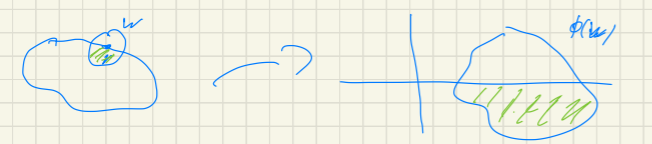
\includegraphics[width=.8\textwidth]{img/IX_1_Plaettung.png}
    \item Subniveau:\\
      $\forall p\in \partial \Omega \ \exists W \subset \mathbb{R}^n$ offen mit $p \in W$ und $h \in C^1(W)$ mit $Dh(q) \neq 0) \\\forall q \in W$, sodass $\Omega \cap W = \{q \in W \ | \ h(q) < 0\}$
    \item Subgraph:\\
      $\forall p \in \partial\Omega \ \exists \script{U} \subseteq \mathbb{R}^{n-1}$ offen $\exists$ offenes Intervall $I \subseteq \mathbb{R} \ \exists C^1$-Funktion $u: \script{U} \to I$, sodass nach geeigneter Umnummerierung der Koordinaten gilt:
      $$\Omega \cap (\script{U} \times I) = \{(x,y) \in \script{U} \times I \ | \ y < u(x)\}$$
  \end{enumerate}
  Die Menge $\Omega$ hat $C^1$-Rand wenn eines (und damit jedes) der drei Kriterien erfüllt ist.
\end{theorem}
\begin{proof}
  siehe Blatt 12
\end{proof}

\begin{lemma}
  In der Situation von Satz IX.1,3) gilt:
  \begin{align*}
    \partial \Omega \cap(\script{U}\times I) &= \{(x,y) \in \script{U} \times I \ | \ y = u(x)\}\\
    (\mathbb{R}\setminus \bar{\Omega}) \cap (\script{U}\times I) &= \{(x,y) \in \mathbb{U} \times I \ | \ y > u(x)\}
  \end{align*}
  $\implies \partial \Omega$ ist $(n-1)$-dimensionale $C^1$-Untermannigfaltigkeit des $\mathbb{R}^n$ nach dem Graphenkriterium bei Untermannigfaltigkeiten.
\end{lemma}
\begin{proof}
  Mit $h: \script{U} \times I \to \mathbb{R}$, $h(x,y) = y-u(x)$ \\
  Vor. $\implies \Omega \cap (\script{U}\times I) = \{ h<0 \}$ \\
  $h$ stetig $\implies \partial \Omega \cap (\script{U}\times I) \subset \{ h=0\}$ \\
  Ist $h(x,y) = 0$ so folgt für $\epsilon$ klein $(x,y-\epsilon)\in\script{U}\times I$ und $h(x,y-\epsilon) = h(x,y) - \epsilon < 0 \rightarrow (x,y-\epsilon)\in\Omega \cap (\script{U}\times I)\\
  \implies (x,y) \in \bar{\Omega}$ und wegen $(x,y) \notin \Omega \implies (x,y) \in \partial\Omega \cap (\script{U}\times I) \implies \partial\Omega \cap (\script{U}\times I) = \{ h=0\}$ \\
  Zweite Aussage folgt aus $\bar{\Omega} = \Omega \cup \partial\Omega$
\end{proof}

\sidenote{Vorlesung 24}{05.02.2021}
\begin{lemma}
  $\Omega \subseteq \mathbb{R}^n$ offen mit $C^1$-Rand. Dann gibt es zu $p \in \partial\Omega$ genau einen Vektor $\nu(p)\in \mathbb{R}^n$ mit
  \begin{enumerate}
    \item $\nu(p) \perp T_p(\partial \Omega)$ und $||\nu(p)|| = 1$
    \item $p + t \nu(p) \notin \Omega$ für $t$ hinreichend klein
  \end{enumerate}
  $\nu:\partial\Omega\to\mathbb{R}^n, n \mapsto \nu(p)$ ist stetig und heißt \textbf{äußere Normale} von $\Omega$.
\end{lemma}

\begin{remark}[Erinnerung: Tangentialraum]
  $\nu \in \mathbb{R}^n$ heißt \textbf{Tangentialvektor} von $M \subseteq R^n, C^1$-Untermannigfaltigkeit in $p\in M$, falls $\gamma:(-\delta, \delta) \to M$ existiert mit $\gamma(0) = p, \gamma'(0) = \nu$\\
  $T_pM = \{$Alle Tangentualvektoren$\}$ $(n-1)$-dimensionaler Untervektorraum.
\end{remark}

\begin{proof}
  Wähle mit Satz IX.1,3) nach ? Umnummerierung der Koordinaten $\Omega \cap (\script{U}\times I) = \{ (x,y)\in \script{U}\times I: y < u(x) \}$ \\
  Sei $q\in \partial\Omega \cap (\script{U}\times I)$ \\
  Lemma IX.2 $\implies f:\script{U} \to \mathbb{R}^n$, $f(x) = (x, u(x))$ ist lokale Para. von $\partial\Omega$ \\
  $T_q(\partial\Omega)$ in $q = (x, u(x))$ hat Basis $(e_i, \frac{\partial u}{\partial x_i}(x)) = \frac{d}{dt} f(x+te_i)|_{t=0}$ für $i=1, ..,n-1$\\
  Definiere auf $\partial\Omega \cap (\script{U}\times I)$ für $q=(x,u(x))$ $$r(q) = \frac{(-Du(x), 1)}{\sqrt{(1+||Du(x)||^2)}}$$
  $\implies r$ erfüllt 1) \\
  Es gilt $q+t r(q) = (x(t),y(t))$ mit $x(t) = x-t\frac{Du(x)}{\sqrt{(1+||Du(x)||^2)}}$, $y(t) = u(x) + t \frac{1}{\sqrt{(1+||Du(x)||^2)}}$ \\
  $\implies \frac{d}{dt} |y(t)-u(x(t))|_{t=0} = \frac{1}{\sqrt{(1+||Du(x)||^2)}} + Du(x) \frac{Du(x)}{\sqrt{(1+||Du(x)||^2)}} = \sqrt{(1+||Du(x)||^2)} > 0$ \\
  Lemma IX.2 $\implies q+t r(q) \notin\Omega$, $q-tr(q)\in\Omega$ für $t$ hinreichend klein \\
  $\implies r\in C^0$ folgt aus $u\in L^1$
\end{proof}
\begin{definition}
  Für $\Omega \subseteq \mathbb{R}^n$ sei $C^1(\bar{\Omega})$ der Unterraum aller $f\in C^1(\Omega)$, für die $f$ und $Df$ stetige Fortsetzungen auf $\partial \Omega$ besitzen. Die \textbf{Fortsetzung} wird wieder mit $f$ bezeichnet.
\end{definition}

\begin{lemma}
  Sei $\Omega = \{(x,y) \in \script{U} \times T \ | \ y<u(x)\}$ wobei $\script{U} \subseteq \mathbb{R}^{n-1}$ offen, $I = (a,b) \subseteq \mathbb{R}$ und $u \in C^1(\script{U}, I)$. Hat $X \in C^1(\bar{\Omega, \mathbb{R}^n})$ kompakten Träger in $\script{U}\times I$, so gilt:
  $$\int\limits_{\Omega} div \ X \ d\lambda^n = \int\limits_{\partial \Omega} <X, \nu> \ d\mu$$
\end{lemma}
\begin{proof}
  $X(x,a) = 0$ $\forall x\in \script{U} \implies \int\limits_\Omega \frac{\partial X_n}{dy} \overset{\text{Fubini}}{=} \int\limits_{\script{U}}\int\limits_u^{u(x)} \frac{\partial X_n}{\partial y} dy dx = \int\limits_{\script{U}} X_n(x,u(x)) dx$ \\
  \item[\underline{Beh}] Für $i=1,...,n-1$ gilt: $\int\limits_\Omega \frac{\partial X_i}{\partial x_i} d\lambda^n = - \int\limits_{\script{U}} X_i(x,u(x))\frac{\partial u}{\partial x_i}dx$ \\
  Damit gilt dann: 
  \begin{align*}
  	\int\limits_\Omega div X d\lambda^n &= -\sum\limits_{i=1}^{n-1} \int \limits_{\script{U}} X_i(x,u(x)) \frac{\partial u}{\partial x_i}(x) dx + \int\limits_{\script{U}} X_n(x,u(x)) dx \\
  	&= \int\limits_{\script{U}} <X(x,u(x)), \frac{(-Du(x),1)}{\sqrt{(1+||Du(x)||^2)}} > \sqrt{(1+||Du(x)||^2)}dx \\
  	&= \int\limits_{\partial\Omega} <X,r> d\mu 
  \end{align*}
  \item[] \underline{Beweis von Beh.} \\
  Sei $\eta \in C^\infty(\mathbb{R})$ mit $\eta(t) = 1$ für $t \leq -2$, $eta(t) = 0$ für $t\geq -1$ und setze $eta_\epsilon (t):= \eta(\frac{t}{\epsilon})$ \\
  $\implies \eta_\epsilon(y-u(x)) = 0$ für $y \geq u(x) - \epsilon$ und $\lim\limits_{\epsilon\to 0} \eta_\epsilon(y-u(x)) = \begin{cases} 1 \text{ falls } y < u(x) \\ 0 \text{ sonst} \end{cases}$ \\
  $\int\limits_\Omega \frac{\partial X_i}{\partial x_i} (x,y) \eta_\epsilon(y-u(x)) d\lambda^n(x,y) = \int\limits_\Omega X_i(x,y) \eta'_\epsilon(y-u(x)) \frac{\partial u}{\partial x_i}(x)d\lambda^n(x,y) = -\int\limits_\Omega \frac{\partial X_i}{\partial y}(x,y) \eta_\epsilon(y-u(x)) \frac{\partial u}{\partial x_i}x_i d\lambda^n(x,y) $ \\
  Alle Funktionen beschränkt $\overset{\text{Lebesgue}, \epsilon\to 0}{\implies}$
  \begin{align*}
  	 \int\limits_\Omega \frac{\partial X_i}{\partial x_i} d\lambda^n &= -\int\limits_\Omega \frac{\partial X_i}{\partial y} (x,y) \frac{\partial u}{\partial x_i} (x) d\lambda^n(x,y) \\
  	 &= -\int\limits_{\script{U}} \left( \int\limits_u^{u(x)} \frac{\partial X_i}{\partial y} (x,y) dy\right) \frac{\partial u}{\partial x_i} dx \\
  	 &= -\int\limits_{\script{U}} X_i (x,u(x)) \frac{\partial u}{\partial x_i} dx
  \end{align*}
\end{proof}

\begin{lemma}
  Sei $W_{\lambda}, \lambda \in \Lambda$, eine offene Überdeckung der kompakten Menge $K \subseteq \mathbb{R}^n$. Dann gibt es eine \textbf{untergeordnete Teilung der Eins}, d.h. es gibt eine endliche Familie von Funktionen $\psi_j \in C_c^{\infty}(\mathbb{R}^n), j \in J$, so dass gilt:
  \begin{enumerate}
    \item $\sum\limits_{j \in J} \psi_j(p) = 1 \ \ \ \forall \ p \in K$
    \item $\forall \ j \in J \ \exists \ \lambda = \lambda(j)$ mit $spt \ \psi_j \subseteq W_{\lambda}$
  \end{enumerate}
\end{lemma}
\begin{proof}
  Wähle eine beschränkte offene Menge $\Omega \supset K$ und bestimme zu jedem $p\in \bar{\Omega}$ einen Ball $b_{r(p)}(p)$ wie folgt: \\
  Für $p\in K$ wähle $\lambda(p)\in \Lambda$ mit $p\in W_{\lambda(p)}$ und weiter $r(p) > 0$ mit $\overline{B_{2r(p)}(p)}\subset (W_{\lambda(p)}\cap \Omega)$. \\
  Für $p\in \bar{\Omega}\setminus K$ wähle $r(p) >0 $ mit $\overline{B_{2r(p)}(p)}\cap K = \varnothing$ endlich viele Kugeln $B_{r(p_j)}$, $1\leq j \leq N$, Überdeckungen $\bar{\Omega}$. Wähle nun $\tilde{\psi_j} \in C^\infty_C(\mathbb{R}^n)$ mit $\tilde{\psi_j} = \begin{cases} 1 \text{ auf } B_{r(p_j)}(p_j) \\ 0 \text{ auf } \mathbb{R}^n\setminus B_{2r(p_j)}(p_j) \end{cases} \\
  \implies \sum\limits_{j=1}^N \tilde{\psi_j} \geq 1$ auf $\bar{\Omega}$. \\
  Die Funktionen $\psi_j = \frac{\tilde{\psi_j}}{\sum\limits_{j=1}^N \tilde{\psi_j}}$ mit $j\in J:=\{j: p_j \in K \}$ sind glatt in $\Omega$ mit $spt \psi_j \subset\subset W_{\lambda(p_k)} \cap \Omega $ wegen $\tilde{\psi_j}|_K = 0$ für $j\notin J$ \\
  $\implies \sum\limits_{j\in J} \psi_j = 1$ auf $K$.
\end{proof}

\begin{theorem}[Integralsatz von Gauß]
  $\Omega \subseteq \mathbb{R}^n$ offen, beschränkt mit $C^1$-Rand und äußere Normale $\nu:\partial\Omega\to\mathbb{R}^n$. Dann gilt für $X\in C^1(\bar{\Omega}, \mathbb{R}^n)$:
  $$\int\limits_{\Omega} div \ X \ d\lambda^n = \int\limits_{\partial\Omega} <X, \nu> \ d\mu$$
\end{theorem}

\begin{remark}
  Gilt auch für Gebiete, deren Rand lokal lipschitz ist (d.h. $u$ in Satz IX.1,3) ist lipschitz (siehe Buch von H.W. Alt: Lineare Funktionalanalysis) \\
  \includegraphics[width=3cm]{img/IX_7_Bem.png}
\end{remark}

\sidenote{Vorlesung 25}{08.02.2021}
\begin{proof}
	Wähle nach Satz IX.1 3) zu jedem $p\in \partial\Omega$ eine Umgebung $W_p$, in der $\Omega$ bzgl geeigneter Koordinaten als Subgraph dargestellt ist. Für $p\in \Omega$ setze einfach $W_p = \Omega \implies \bigcup\limits_{p\in\bar{\Omega}} W_p \supset \bar{\Omega}$ und $W_p$ sind offen $\forall p\in \bar{\Omega}$ \\
	Lemma IX.6 $\implies\exists$ untegeordnete Zerlegung der 1 $\psi_1, ..., \psi_N \in C^\infty_C (\mathbb{R}^n)$. \\
	Liegt $spt \psi_j$ in einer Randumgebung $W_p = \script{U}\times I$ wie in Satz IX.1 3), so folgt aus Lemma IX.5 $$ \int\limits_\Omega div (\psi_j X) dx = \int\limits_{\partial\Omega} < \psi_j X, v> d\mu$$
	Ist $spt \psi_j \in \Omega$, so folgt mit part. Integration $$\int\limits_\Omega div(\psi_j X) dx = 0 = \int\limits_{\partial\Omega} <\psi_j X, v> d\mu$$ 
	$\implies \int\limits_\Omega div X dx = \sum\limits_{j=1}^N \int\limits_\Omega div(\psi_j X) dx = \sum\limits_{j=1}^N \int\limits_{\partial\Omega} <\psi_j X, v> d\mu = \int\limits_{\partial\Omega}<X,v> d\mu$
\end{proof}
\begin{example}
  Wähle $X(x) = x \implies \lambda^n(\Omega) = \frac{1}{n} \int\limits_{\Omega} div \ X \ dx = \frac{1}{n} \int\limits_{\partial \Omega} <x, \nu(x)> \ d\mu(x)$\\
  Speziell: $\alpha = \frac{\omega_{n-1}}{n}$\\
  $\Omega = B_1(0) \subseteq \mathbb{R}^n \rightarrow \nu(x) = x, \partial\Omega = S^{n-1}$ 
\end{example}

\begin{lemma}[Greensche Formeln]
  $\Omega \subseteq \mathbb{R}^n$ offen und beschränkt mit $C^1$-Rand. Dann gilt für $u \in C^1(\bar{\Omega})$ und $v \in C^2(\bar{\Omega})$
  \begin{enumerate}
    \item $\int\limits_{\Omega}(u \triangle v + <\triangledown u, \triangledown v>) \ d\lambda^n = \int\limits_{\partial \Omega} u \frac{\partial v}{\partial \nu} \ d\mu \ \ \ (\frac{\partial v}{\partial \nu} = <\triangledown v, \nu>)$
  \end{enumerate}
  Weiter folgt für $u,v \in C^2(\bar{\Omega})$
  \begin{enumerate}[resume]
    \item $\int\limits_{\Omega} (u \triangle v - v \triangle u) \ d\lambda^n = \int\limits_{\partial \Omega}(u \frac{\partial v}{\partial \nu} - v \frac{\partial u}{\partial \nu}) \ d\mu$
  \end{enumerate}
\end{lemma}

\begin{proof}
  \item[1)] Benutze $div(u\triangledown v) = <\triangledown u, \triangledown v> + u \triangle v$ \\
  Gauss $\implies \int\limits_{\partial\Omega} <u\triangledown v,v> d\mu = \int\limits_\Omega div(u \triangledown v) d\lambda^n = \int\limits_\Omega (<\triangledown u, \triangledown v> + u \triangle v) d\lambda^n$
  \item[2)] 1) $\implies \int (v\triangle u + <\triangledown v, \triangledown u>) d\lambda^n = \int\limits_{\partial\Omega} v \frac{\partial u}{\partial v} d\mu$ \\
  Bilde Differenz $\implies$ 2)
\end{proof}

\begin{example}
  \underline{Mittelwerteigenschaft harmonischer Funktionen}\\
  Sei $\mu \in C^2(\Omega)$ eine \textbf{harmonische Funktion}, d.h. $\triangle u = 0$ in $\Omega$.\\
  Für $x_0 \in \Omega$ und $0<r<dist(x_0, \partial \Omega)$ gilt:
  $$\int\limits_{\partial B_r(x_0)} \frac{\partial u}{\partial \nu} \ d\mu \stackrel{\text{Gauß}}{=} \int\limits_{B_r(x_0)} \triangle u \ d\lambda^n = 0 \ \ \ \ \ \triangle u = div \ (\triangledown u)$$
  Auf $\mathbb{R}^n\setminus\{x_0\}$ betrachte weiter $v(x) = \gamma(||x-x_0||)$ mit $\gamma(\rho) = \begin{cases}
    \frac{\rho^{2-n}}{2-n} & , n\geq 3\\
    \log(\rho) & , n = 2
  \end{cases}$\\
  $\stackrel{\text{Ana II}}{\implies} v$ ist harmonisch auf $\mathbb{R}^n\setminus\{x_0\}$\\
  \\
  ... Rest siehe Aufschrieb
\end{example}

\begin{example}
  siehe Aufschrieb
\end{example}
  \chapter{Faltung und Fouriertransformation}
\begin{theorem}
	Sei $f\in L^p(\mathbb{R}^n)$, $1\leq p \leq \infty$ und $g\in L^1(\mathbb{R}^n)$. \\
	Die Faltung von $f$ mit $g$ ist die $\lambda^n$-fast überall definierte Funktion 
	$$ f\ast g: \mathbb{R}^n \to \mathbb{\bar{R}}\text{, } (f\ast g)(x) = \int\limits_{\mathbb{R}^n} f(x-y) g(y) dy $$
	Es gilt $f\ast g\in L^p(\mathbb{R}^n)$ mit $||f\ast g||_{L^p} \leq ||f||_{L^p} ||g||_{L^1}$
\end{theorem}
\begin{proof}
Aufschrieb
\end{proof}

\begin{lemma}
	$f\in L^p(\mathbb{R}^n)$ mit $1\leq p \leq \infty$ und $\tau_h: \mathbb{R}^n\to \mathbb{R}^n$, $\tau_h(x)=x+h$. Dann gelten:
	\item[i)] $f\circ \tau_h \in L^p(\mathbb{R}^n)$ mit $||f\circ \tau_h ||_{L^p} = ||f||_{L^p}$
	\item[ii)] $f\circ \tau_h \to f$ in $L^p(\mathbb{R}^n)$ für $h\to 0$, falls $1\leq p < \infty$
\end{lemma}
\begin{proof}
	\item[i)] Trivial
	\item[ii)] s. Blatt 9, Aufgabe 1
\end{proof}

\begin{theorem}
	$f\in L^p(\mathbb{R}^n)$ mit $ 1\leq p \leq \infty$. Ist $\eta \in L^1(\mathbb{R}^n)$ mist $\int\limits_{\mathbb{R}^n} \eta(z) dz = 1$, so folgt $\eta_\rho (x) = \rho^{-n} \eta(\frac{x}{\rho})$: 
	\begin{equation*}
		||f\ast \eta_\rho||_{L^p} \leq ||f||_{L^p} ||\eta||_{L^1} \\
		\text{ und } \\
		f\ast \eta_\rho \to f \text{ in } L^p(\mathbb{R}^n) \text{ für } \rho \to 0
	\end{equation*}
\end{theorem}

\begin{proof}
	siehe Aufschrieb
\end{proof}

\begin{theorem}
	Sei $\eta \in C^k(\mathbb{R}^n)$ mit $|| D^\alpha \eta ||_{C^0(\mathbb{R}^n)} \leq C_k$ für $|\alpha| \leq k$ $(\alpha = (\alpha_1, ..., \alpha_n), |\alpha| = \alpha_1+...+\alpha_n, D^\alpha = \partial_1^{\alpha_1}\cdot ... \cdot \partial_n^{\alpha_n})$. Für $f \in L^1(\mathbb{R}^n)$ ist dann $f\ast \eta \in C^k(\mathbb{R}^n)$ und es gilt $D^\alpha (f\ast \eta) = f\ast (D^\alpha \eta)$, speziell $||D^\alpha(f\ast \eta)||_{C^0(\mathbb{R}^n)} \leq C_k ||f||_{L^1}$
\end{theorem}
\begin{proof}
	siehe Aufschrieb
\end{proof}

\begin{theorem}
	$\Omega \subset\mathbb{R}^n$ offen und $1\leq p < \infty$. Dann ex. zu $f\in L^p(\Omega)$ eine Folge $f_k \in C^\infty_C(\Omega)$ mit $||f-f_k||_{L^p}\to 0$ mit $k \to \infty$. 
\end{theorem}
\begin{proof}
	siehe Aufschrieb
\end{proof}

\begin{definition}
	Die Fourier-Transformierte von $f\in L^1(\mathbb{R}^n, \mathbb{C})$ ist die Funktion 
	$$\hat{f}: \mathbb{R}^n \to \mathbb{C}\text{, } \hat{f}(p) = (2\pi)^{-\frac{n}{2}} \int\limits_{\mathbb{R}^n} f(x) \text{e}^{-i<p,x>}dx$$
	Die Inverse Fourier-Transformierte von $g\in L^1(\mathbb{R}^n, \mathbb{C})$ ist $$
	\check{g}:\mathbb{R}^n \to \mathbb{C}\text{, } \check{g}(x) = (2\pi)^{-\frac{n}{2}} \int\limits_{\mathbb{R}^n} g(p) \text{e}^{i<p,x>}dp$$
\end{definition}

\begin{theorem}
	Für $f,g\in L^1(\mathbb{R}^n,\mathbb{C})$ gilt:
	\item[1)] $\hat{f}\in C^0(\mathbb{R}^n,\mathbb{C})$ und $||\hat{f}||_{C^0(\mathbb{R}^n)} \leq (2\pi)^{-\frac{n}{2}}||f||_{L^1}$
	\item[2)] $\widehat{f\ast g} = (2\pi)^{\frac{n}{2}}\hat{f}\hat{g}$
	\item[3)] $<\hat{f},g>_{L^2(\mathbb{R}^n)} = < f,\check{g}>_{L^2(\mathbb{R}^n)}$
\end{theorem}
\begin{proof}
	siehe Aufschrieb 
\end{proof}

\begin{example}
	siehe Aufschrieb
\end{example}

\begin{theorem}[Plancherel]
	Für $f\in (L^1\cap L^2)(\mathbb{R}^n,\mathbb{C})$ gilt $||\hat{f}||_{L^2} = ||\check{f}||_{L^2} = ||f||_{L^2}$
\end{theorem}

\begin{proof}
	siehe Aufschrieb
\end{proof}

\begin{theorem}
	Es gibt eine eindeutig bestimmte Abb. $\script{F}, \script{F}^\ast: L^2(\mathbb{R}^n,\mathbb{C}) \to L^2(\mathbb{R}^n,\mathbb{C})$ mit
	\item[1] $\script{F}f = \hat{f}$, $\script{F}^\ast f = \check{f}$ $\forall f\in (L^1\cap L^2)(\mathbb{R}^n,\mathbb{C})$
	\item[2] $||\script{F}f||_{L^2} = ||f||_{L^2} = ||\script{F}^\ast f||_{L^2}$ $\forall f\in L^2(\mathbb{R}^n,\mathbb{C})$ 
	Weiter gelten für $f,g\in L^2(\mathbb{R}^n,\mathbb{C})$ 
	\item[3] $<\script{F}f,\script{F}g>_{L^2} = <f,g>_{L^2} = <\script{F}^\ast f, \script{F}^\ast g>_{L^2}$
	\item[4] $<\script{F}f,g> _{L^2} = <f,\script{F}^\ast g>_{L^2}$
	\item[5] $\script{F}^\ast \script{F} = \script{F} \script{F}^\ast = \text{Id}_{L^2(\mathbb{R}^n)}$
\end{theorem}
\begin{proof}
	siehe Aufschrieb
\end{proof}

\begin{notation} 
	$\script{F}f = \hat{f}$, $\script{F}^\ast f = \check{f}$ auch wenn $f,g$ nur in $L^2$
\end{notation}

\begin{definition}[Schwartz-Raum]
	$S(\mathbb{R}^n,\mathbb{C}) = \{f\in C^\infty (\mathbb{R}^n,\mathbb{C}): x^\alpha D^\beta f$ ist beschränkt für alle $\alpha,\beta \in \mathbb{N}^n_0 \}$ \\
	$(x^\alpha = x_1^{\alpha_1}... x_n^{\alpha_n}), D^\beta = \partial_1^{\beta_1}...\partial_n^{\beta_n}$
\end{definition}

\begin{remark}
	$f\in S(\mathbb{R}^n,\mathbb{C}) \implies |f(x)| \leq c_N (1+||x||^2)^{-\frac{N}{2}}$ $\forall N\in \mathbb{N}$ \\
	$\implies f\in L^p(\mathbb{R}^n,\mathbb{C})$ $\forall p\in [1,\infty]$ \\
	Außerdem: $f\in S(\mathbb{R}^n,\mathbb{C}) \implies \partial_j f$ und $x_jf \in S(\mathbb{R}^n,\mathbb{C})$ $\forall 1\leq j \leq n$
\end{remark}

\begin{theorem}
	Mit $f$ ist auch $\hat{f}\in S(\mathbb{R}^n,\mathbb{C})$ und 
	\item[1)] $\widehat{\partial_j f}(p) = i p_j \hat{f}(p)$ sowie $\widehat{x_j f}(p) = i \partial_j \hat{f}(p)$
	\item[2)] $f(x) = (2\pi)^{-\frac{n}{2}}\int\limits_{\mathbb{R}^n} \hat{f}(p) \text{e}^{i<p,x>}dp$ $\forall x\in \mathbb{R}^n$
\end{theorem}
\begin{proof}
	siehe Aufschrieb
\end{proof}

\begin{example}
	siehe Aufschrieb
\end{example}
  
\end{document}